\pdfoutput=1
\pdfminorversion=7
\documentclass[11pt]{article}

\usepackage[review]{acl}
\usepackage{times}
\usepackage{latexsym}
\usepackage[T1]{fontenc}
\usepackage[utf8]{inputenc}
\usepackage{microtype}
\usepackage{inconsolata}
\usepackage{graphicx}
\usepackage{booktabs}
\usepackage{multirow}
\usepackage{makecell}
\usepackage{array}
\usepackage{tabularx}
\usepackage{amsmath}
\usepackage{amssymb}
\usepackage{xcolor}
\usepackage{enumitem}
\usepackage[most]{tcolorbox}
\usepackage{placeins}

\graphicspath{{../../figures/llama8b/pdf/}{../../figures/qwen/pdf/}{../../figures/llama70b/pdf/}}

\newcommand{\diy}{\textsc{DebiasItYourself}}
\newcommand{\llama}{\textsc{Llama}}
\newcommand{\qwen}{\textsc{Qwen}}
\newcommand{\sr}{\textsc{SR}}
\newcommand{\ci}{\textsc{CI}}
\newcommand{\ind}{\textsc{IND}}
\newcommand{\pt}{\textsc{PT}}
\newcommand{\pc}{\textsc{PC}}
\newcommand{\todo}[1]{\textcolor{red}{[#1]}}

% Highlight styles use the reference-paper structure with a DIY-specific palette.
\definecolor{diyInsightBg}{HTML}{E7F1F0}
\definecolor{diyInsightRule}{HTML}{347C78}
\definecolor{diyBaseBg}{HTML}{DDE3EC}
\definecolor{diyIclBg}{HTML}{BFE1F4}
\definecolor{diyItBg}{HTML}{F4BFD3}
\definecolor{diyNoItBg}{HTML}{BFE7CE}
\definecolor{diyTpItBg}{HTML}{F8DA82}
\definecolor{diySrBg}{HTML}{F3B6A9}
\definecolor{diyCiBg}{HTML}{B6D8F3}
\definecolor{diyIndBg}{HTML}{BEE8CD}
\definecolor{diyPtBg}{HTML}{F2CD79}
\definecolor{diyPcBg}{HTML}{D1BDF0}
\definecolor{diyBadgeBorder}{HTML}{3E4654}

\newtcolorbox{insightbox}{
  enhanced,
  colback=diyInsightBg,
  colframe=diyInsightRule,
  boxrule=0pt,
  leftrule=5pt,
  rightrule=0pt,
  toprule=0pt,
  bottomrule=0pt,
  sharp corners,
  fontupper=\small,
  before skip=5pt,
  after skip=5pt,
  top=3pt,
  bottom=3pt,
}
\let\takeawaybox\insightbox
\let\endtakeawaybox\endinsightbox

\newcommand{\tabstrut}{\rule{0pt}{2.8ex}}

\newcommand{\highlightRounded}[2]{%
  \begin{tikzpicture}[baseline=(word.base)]
    \node[
      rectangle,
      rounded corners,
      fill=#1,
      draw=diyBadgeBorder,
      line width=0.55pt,
      inner sep=2pt
    ] (word) {#2};
  \end{tikzpicture}%
}

\newcommand{\highlightRoundedBorder}[2]{%
  \begin{tikzpicture}[baseline=(word.base)]
    \node[
      rectangle,
      rounded corners,
      fill=#1,
      draw=diyBadgeBorder,
      line width=0.5pt,
      inner sep=2pt
    ] (word) {#2};
  \end{tikzpicture}%
}

\newcommand{\baseinfer}{\highlightRounded{diyBaseBg}{\textsc{Base}}}
\newcommand{\icllabel}{\highlightRoundedBorder{diyIclBg}{\textsc{ICL}}}
\newcommand{\diyit}{\highlightRounded{diyItBg}{\diy{} IT}}
\newcommand{\diynoit}{\highlightRoundedBorder{diyNoItBg}{\diy{} Two Pass (No IT)}}
\newcommand{\diytpit}{\highlightRoundedBorder{diyTpItBg}{\diy{} Two Pass (IT)}}
\newcommand{\srfull}{\textsc{Stereotype Replacement}}
\newcommand{\cifull}{\textsc{Counter-stereotypic Imaging}}
\newcommand{\indfull}{\textsc{Individuation}}
\newcommand{\ptfull}{\textsc{Perspective-taking}}
\newcommand{\pcfull}{\textsc{Positive Contact}}

\title{\diy{}: Structured Supervision for Generalizable Bias-Reducing Interventions}

\author{
  Anonymous EMNLP submission
}

\begin{document}
\maketitle

\begin{abstract}
Large language models often handle bias-sensitive context as if social salience were task evidence: names, group descriptors, roles, occupations, events, and institutions can become shortcuts even when they are irrelevant to the correct answer. We introduce \diy{}, a structured supervision method for teaching reusable bias-reducing behavior. \diy{} translates prejudice-reducing interventions from social psychology into model-facing supervision, covering \srfull{}, \cifull{}, \indfull{}, \ptfull{}, and \pcfull{}. The contribution is not a new prompt template or a psychology label attached to fine-tuning; the intervention inventory defines a shared training and inference schema for identifying unsupported social assumptions and producing task-consistent outputs. We evaluate \diy{} across CrowS-Pairs, StereoSet, BBQ, WinoBias, and WinoGender, using normalized bias error so that lower values consistently indicate better mitigation. We compare \diyit{}, \icllabel{}, and \diy{} two-pass inference against a broad set of debiasing baselines, and we evaluate Balanced COPA and ARC to test whether bias reduction preserves reasoning competence. Across the current results, \diy{} improves cross-benchmark bias error most consistently when intervention-guided inference is paired with structured supervision, while companion \qwen{} and \llama{}-70B analyses suggest that the same pattern is not tied to a single model family.
\end{abstract}

\section{Introduction}
\label{sec:introduction}

Language models are trained on text that is saturated with social information. Names, demographic descriptors, occupations, institutions, events, neighborhoods, dialectal cues, and interpersonal roles all appear in contexts shaped by historical asymmetries and cultural stereotypes. These cues are often useful for understanding a task, but they can also become shortcuts. A model may treat a role as evidence of competence, an occupation as evidence of gender, a group descriptor as evidence of behavior, or a social situation as evidence for blame. The resulting failure is not only that models encode biased associations. A model may know that stereotyping is undesirable and still fail to decide, in context, whether a social cue is relevant evidence, irrelevant background, or an unsupported heuristic.

This distinction matters for bias mitigation. A good model should not simply erase social information or refuse to answer whenever a sensitive cue appears. Sometimes the cue is irrelevant and should not affect the answer. Sometimes it is relevant but must be grounded in the evidence provided by the task. Sometimes the input invites a stereotyped inference that should be revised. In other cases, the model should preserve the task objective while avoiding generic moralizing or over-sanitized language. Across likelihood benchmarks, ambiguous question answering, coreference, and generation, the same underlying challenge appears: the model must handle bias-sensitive context without letting social salience become social evidence.

Most existing mitigation pipelines intervene through a particular mechanism: counterfactual augmentation, parameter-efficient fine-tuning, activation steering, decoding constraints, preference optimization, or prompt-based self-revision. These mechanisms are valuable, but the mechanism itself is rarely a sufficient theory of the behavior the model should learn. A method that improves a pairwise likelihood benchmark may not teach the model how to answer an ambiguous question. A method that reduces a stereotype score may do so by becoming vague, evasive, or less useful. A method tuned around one bias category may not define what to do when the cue changes from an identity term to an occupation, a social role, or a contextual relation.

\diy{} starts from a different technical premise: the core object of debiasing should be the bias-reducing behavior the model learns, not the delivery mechanism used to induce it. We define bias mitigation as learning intervention-guided response generation. Given an input that may invite an unsupported social shortcut, the model must produce an output justified by task evidence rather than by stereotype, salience, or majority priors. The intervention inventory is motivated by the prejudice habit-breaking intervention of \citet{devine2012longterm}, which teaches concrete bias-reducing procedures such as \srfull{}, \cifull{}, \indfull{}, \ptfull{}, and \pcfull{}. We do not claim that language models possess implicit attitudes in the human psychological sense. Instead, we translate these procedures into model-facing supervision: each intervention specifies what evidence to attend to, what heuristic to avoid, and what kind of task-consistent output to produce.

\diy{} implements this premise as a single structured supervision method. It constructs a broad set of biased and debiased instances, labels each debiased target with the intervention that explains the desired behavior, and uses the resulting data to teach intervention-guided revision and response generation. Prompting, fine-tuning, soft prompting, and self-revision are treated as interfaces to the same supervision signal. This distinction matters for the paper's claim: the contribution is not psychology plus fine-tuning, but a method for teaching models how to handle bias-sensitive context through reusable bias-reducing interventions.

Our central claim is deliberately scoped:
\begin{insightbox}
\textbf{Paper thesis.} \diy{} teaches language models to handle bias-sensitive context as evidence-grounded input rather than as a social shortcut, using reusable intervention-guided behaviors.
\end{insightbox}
The paper evaluates this claim through three questions:
\begin{enumerate}[leftmargin=1.4em,itemsep=1pt,topsep=2pt]
    \item Does \diy{} reduce bias across multiple datasets rather than only on the data format used to construct its supervision?
    \item Which components matter: intervention labels, mixtures of interventions, rationales, and the interface used to provide supervision?
    \item Does \diy{} preserve reasoning performance, or does stronger debiasing trade away task competence?
\end{enumerate}

We make four contributions.
\begin{enumerate}[leftmargin=1.4em,itemsep=1pt,topsep=2pt]
    \item We formalize bias mitigation as structured debiasing supervision, rather than as a benchmark-specific post-hoc patch.
    \item We construct a data generation pipeline that pairs biased instances with intervention-labeled debiased targets across social categories, instance types, and domains.
    \item We instantiate \diy{} through training-time and inference-time interfaces, using these variants as ablations of one method rather than separate methods.
    \item We compare \diy{} against a broad set of debiasing baselines across bias and reasoning benchmarks, explicitly measuring generalization across evaluation settings and utility preservation.
\end{enumerate}

\section{Related Work}
\label{sec:related-work}

\paragraph{Bias benchmarks.}
CrowS-Pairs evaluates whether a model assigns higher likelihood to stereotypical than anti-stereotypical sentence pairs across multiple social bias categories \citep{nangia-etal-2020-crows}. StereoSet measures stereotypical associations while also tracking language modeling ability through ICAT-style scoring \citep{nadeem-etal-2021-stereoset}. BBQ evaluates social bias in question answering by comparing model behavior in ambiguous and disambiguated contexts \citep{parrish-etal-2022-bbq}. WinoBias and WinoGender study gender bias in coreference and occupation-linked schemas \citep{zhao-etal-2018-gender,rudinger-etal-2018-gender}. Additional evaluations such as HONEST, UNQOVER, BOLD, and Bias in Bios broaden the task surface to hurtful completions, underspecified questions, open-ended generation, and occupation prediction \citep{nozza-etal-2021-honest,li-etal-2020-unqovering,PLACEHOLDER_bold_verify,PLACEHOLDER_biasbios_verify}. \diy{} uses this diversity as an evaluation requirement: a mitigation method should not be judged from one benchmark alone.

\paragraph{Bias mitigation in language models.}
Prior work has explored mitigation at several points in the modeling pipeline, including data augmentation, representation editing, parameter-efficient fine-tuning, activation steering, preference optimization, prompt-based revision, and decoding-time control. Self-diagnosis and self-debiasing methods ask models to recognize and reduce their own toxic or biased continuations without additional training data \citep{PLACEHOLDER_schick_selfdebias_verify}. Empirical surveys show that debiasing methods can produce inconsistent effects across benchmarks and may reduce language modeling or downstream performance \citep{PLACEHOLDER_meade_survey_verify}. \diy{} is complementary to the mechanism-level view: it specifies the supervision signal a mitigation method should induce. The implementation mechanism is then an interface to the same structured supervision, not the main scientific unit.

\paragraph{Identity coverage.}
Many bias datasets focus on a small number of axes, often gender, race, or religion. HolisticBias expands descriptor coverage to a broader set of demographic axes and emphasizes participatory construction of identity descriptors \citep{smith-etal-2022-im}. \diy{} uses broad identity coverage during generation so that the intervention is not tied to one social category. This broad coverage is necessary for our generalization claim but also increases the need for careful safety review, because synthetic biased examples can reproduce harmful language even when used for mitigation.

\paragraph{Prejudice-reducing interventions as supervision design.}
The prejudice habit-breaking intervention treats implicit bias as a habit that can be changed through awareness, concern, and repeated use of bias-reducing procedures \citep{devine2012longterm}. The five interventions are not merely labels; they describe distinct behaviors for reducing biased responses. \srfull{} identifies and substitutes a biased response. \cifull{} makes non-stereotypical exemplars salient. \indfull{} shifts attention from group membership to person-specific evidence. \ptfull{} asks the reasoner to consider the affected person's experience. \pcfull{} increases exposure to counter-stereotyped, constructive intergroup examples. \diy{} adapts these intervention ideas into model-facing supervision, prompts, and inference-time revisions.

\section{Method}
\label{sec:method}

\subsection{Problem Formulation}
\label{sec:problem-formulation}

Let $x$ denote an input that may invite a stereotyped or unsupported group-based inference, and let $y$ denote the desired task output. Standard mitigation methods typically optimize for a narrow proxy: reduce a benchmark score, avoid a set of words, or steer a representation away from a bias direction. \diy{} instead learns intervention-guided response generation:
\[
    p_\theta(y \mid x, b),
\]
where $b$ is a bias-reducing intervention label. The label specifies the desired debiasing behavior for the instance. In this formulation, a debiased output is not merely less toxic or less stereotypical; it must be consistent with the task evidence and the selected intervention.

The training signal for \diy{} consists of triples $(x, b, y_b)$, where $y_b$ is a debiased answer or revision produced under intervention $b$. Optional rationales $r_b$ expose the intermediate reasoning:
\[
    x \xrightarrow{\;b\;} (r_b, y_b), \quad b \in \{\sr,\ci,\ind,\pt,\pc\}.
\]
The rationale is used as supervision or prompting context when helpful, but the central object is the conditional distribution over debiased outputs.

\subsection{Bias-Reducing Interventions}
\label{sec:intervention-formalization}

The five interventions form a structured space of debiasing behaviors. They are deliberately overlapping: many biased instances can be revised in more than one way, but each intervention emphasizes a different failure mode. This gives \diy{} two technical advantages. First, it can supervise multiple valid debiased outputs for the same social bias pattern. Second, it can expose which intervention transfers to which benchmark family.

\begin{table*}[t]
\centering
\footnotesize
\setlength{\tabcolsep}{4pt}
\renewcommand{\arraystretch}{1.12}
\begin{tabularx}{\textwidth}{@{}p{0.31\textwidth}p{0.20\textwidth}p{0.27\textwidth}p{0.16\textwidth}@{}}
\toprule
Intervention & Human intervention idea & Model-facing behavior & Expected failure mode \\
\midrule
\srfull{} & Notice a stereotypic response and replace it with a non-stereotypic response. & Identify biased association, label why it is unsupported, and rewrite or answer without the stereotype. & Overly generic refusal or moralizing without task completion. \\
\cifull{} & Make counter-stereotypic exemplars salient. & Introduce examples that violate the biased association while preserving task content. & Token replacement without deeper reasoning. \\
\indfull{} & Attend to person-specific evidence rather than group-level assumptions. & Prefer contextual evidence over identity priors in QA, coreference, and likelihood comparisons. & Ignoring relevant identity context when it is genuinely task-relevant. \\
\ptfull{} & Consider the experience of the affected person or group. & Simulate the impact of a biased assumption and revise the response accordingly. & Producing verbose empathy language instead of concise answers. \\
\pcfull{} & Increase constructive exposure to out-group members. & Generate balanced, non-tokenizing interactions involving identities across contexts. & Sanitized examples that lack stereotype contrast. \\
\bottomrule
\end{tabularx}
\caption{The five bias-reducing interventions in \diy{}. They define the structured supervision used for data generation, model conditioning, and ablation analysis. This table is a draft placeholder; final wording should be tightened after method review.}
\label{tab:strategies}
\end{table*}

\subsection{Data Generation Pipeline}
\label{sec:data-generation}

\diy{} constructs intervention-labeled supervision in four stages.
First, we build an identity inventory spanning multiple demographic dimensions, drawing from HolisticBias descriptors and generated identity lists. Second, we generate biased seed instances that cover several textual forms: direct statements, short stories, dialogue, news-style snippets, and questions. Third, for each seed instance we generate debiased targets under the five interventions. Fourth, we filter and format these triples into a unified instruction schema:
\[
\begin{aligned}
    &\texttt{Input: }x,\quad \texttt{Intervention: }b,\\
    &\texttt{Debiased output: }y_b.
\end{aligned}
\]
When rationales are used, they are represented as an auxiliary field rather than a separate method.

The generation pipeline explicitly separates three dimensions:
\begin{enumerate}[leftmargin=1.4em,itemsep=1pt,topsep=2pt]
    \item \textbf{Identity dimension}: age, disability, gender identity, nationality, physical appearance, race/ethnicity, religion, sexual orientation, socioeconomic status, and intersections available in the benchmark.
    \item \textbf{Instance type}: opinion, action, event, story, dialogue, news-style text, or question.
    \item \textbf{Bias-reducing intervention}: \srfull{}, \cifull{}, \indfull{}, \ptfull{}, or \pcfull{}.
\end{enumerate}
This design lets us test whether training on intervention-labeled examples transfers beyond the exact surface form used during generation.

\subsection{\diy{} Instantiations}
\label{sec:deployment}

The primary implementation of \diy{} trains or conditions a model on the intervention-labeled supervision above. Different instantiations answer different technical questions about where the supervision should enter the modeling pipeline.

\paragraph{Fine-tuned \diy{}.}
The main trained variant fine-tunes \llama{} models with LoRA on intervention-labeled source/target triples. We evaluate both intervention-specific adapters and all-intervention mixtures. The mixture is the central \diy{} model because it learns a shared representation of bias-reducing behavior across multiple intervention types.

\paragraph{Inference-time \diy{}.}
The inference-time variant conditions the model with the same intervention schema at evaluation time. This tests how much of \diy{} can be activated without parameter updates and whether lightweight conditioning is sufficient for transfer.

\paragraph{Soft-prompt \diy{}.}
Soft-prompt variants learn continuous prompt parameters for the intervention-labeled supervision. This isolates whether the debiasing behavior can be represented in a small learned conditioning vector.

\paragraph{Self-revising \diy{}.}
Self-revising variants ask the model to first answer, then revise the answer under a selected intervention. This is an inference-time realization of the same structured supervision and is useful for tasks where a second pass can explicitly diagnose an unsupported group heuristic.

\paragraph{Ablation variants.}
In-context demonstrations, instruction-only prompts, chain-of-thought variants, sample-size variants, and source-form variants are ablations of \diy{}. They test whether performance depends on demonstrations, rationales, intervention labels, data volume, or the textual form of generated supervision.

\section{Experimental Setup}
\label{sec:setup}

\subsection{Models}
\label{sec:models}

The main experiments use \llama{}-family causal language models, with \llama{} 8B as the primary model because it has the most complete bias, baseline, intervention, shot, and reasoning result matrix. We include \qwen{} and \llama{}-70B companion runs to test whether the same intervention interfaces behave similarly under alternative model families and scales. These companion results are used as robustness evidence rather than as the sole basis for aggregate claims. The camera-ready version should report the exact checkpoints, quantization settings, adapter merge procedure, and decoding settings for each model family.

\subsection{Bias Evaluation}
\label{sec:bias-eval}

We evaluate on five primary bias benchmarks:
\begin{itemize}[leftmargin=1.4em,itemsep=1pt,topsep=2pt]
    \item \textbf{CrowS-Pairs}: stereotype preference should move toward 50.
    \item \textbf{StereoSet}: ICAT score should increase while stereotype score moves toward the neutral point.
    \item \textbf{BBQ}: accuracy should remain high while ambiguous and disambiguated bias scores move toward zero.
    \item \textbf{WinoBias}: gender-linked coreference bias should decrease.
    \item \textbf{WinoGender}: occupation-linked gender bias should decrease.
\end{itemize}
All main figures convert these benchmark-specific metrics into \emph{bias error}, so lower values are consistently better: CrowS-Pairs stereotype preference and StereoSet SS overall are measured as distance from $50$, while BBQ ambiguous/disambiguated bias scores, WinoBias absolute pro--anti gap, and WinoGender male--female pair disagreement are measured as distance from $0$. The appendix includes companion-model plots and missing-data audits for \qwen{} and \llama{}-70B.

\subsection{Baselines}
\label{sec:baselines}

We compare against a broad set of baselines implemented in the repository: DPO-style preference training, BIASEDIT, FairSteer, LFTF, PEFT, BiasFreeBench, BBA, CAL, Debias-NLG, MBIAS, Debias-LLMs, Reduce Social Bias, DeCAP, and self-debiasing reprompting. These baselines cover training-time, representation-level, prompting, and inference-time mitigation families. The comparison is designed to test whether \diy{}'s structured debiasing supervision provides better cross-benchmark behavior than methods defined primarily by a single mitigation mechanism. The final version should include a one-to-one mapping from every baseline label in the figures to its source paper, implementation, and hyperparameter setting.

\subsection{Reasoning Evaluation}
\label{sec:reasoning-eval}

Bias reduction is not sufficient if the method degrades ordinary task competence. We therefore evaluate reasoning and knowledge tasks using Balanced COPA, ARC-Challenge, and ARC-Easy. These evaluations compare \baseinfer{}, \icllabel{}, \diyit{}, \diynoit{}, and \diytpit{}. For the primary \llama{} 8B setting, we use the full reasoning matrix in the main paper. For \qwen{} and \llama{}-70B, we report companion reasoning and bias--utility plots in the appendix.

\section{Results}
\label{sec:results}

\subsection{Debiasing performance}
\label{sec:results-debiasing-performance}

We first ask whether the main \diy{} variants reduce bias across the full benchmark suite, rather than only under one favorable metric. Since the benchmarks report incompatible raw quantities, we plot each benchmark as a \emph{bias error}: distance from the unbiased target. For CrowS-Pairs and StereoSet, the unbiased target is $50$; for BBQ, WinoBias, and WinoGender, the unbiased target is $0$. Lower values are therefore better in every panel.
Unless otherwise stated, the main results in this section are from the \llama{} 8B run matrix, which is the only matrix currently complete across all three axes needed for the central comparison: bias benchmarks, baseline families, and reasoning benchmarks.

\begin{figure*}[t]
\centering
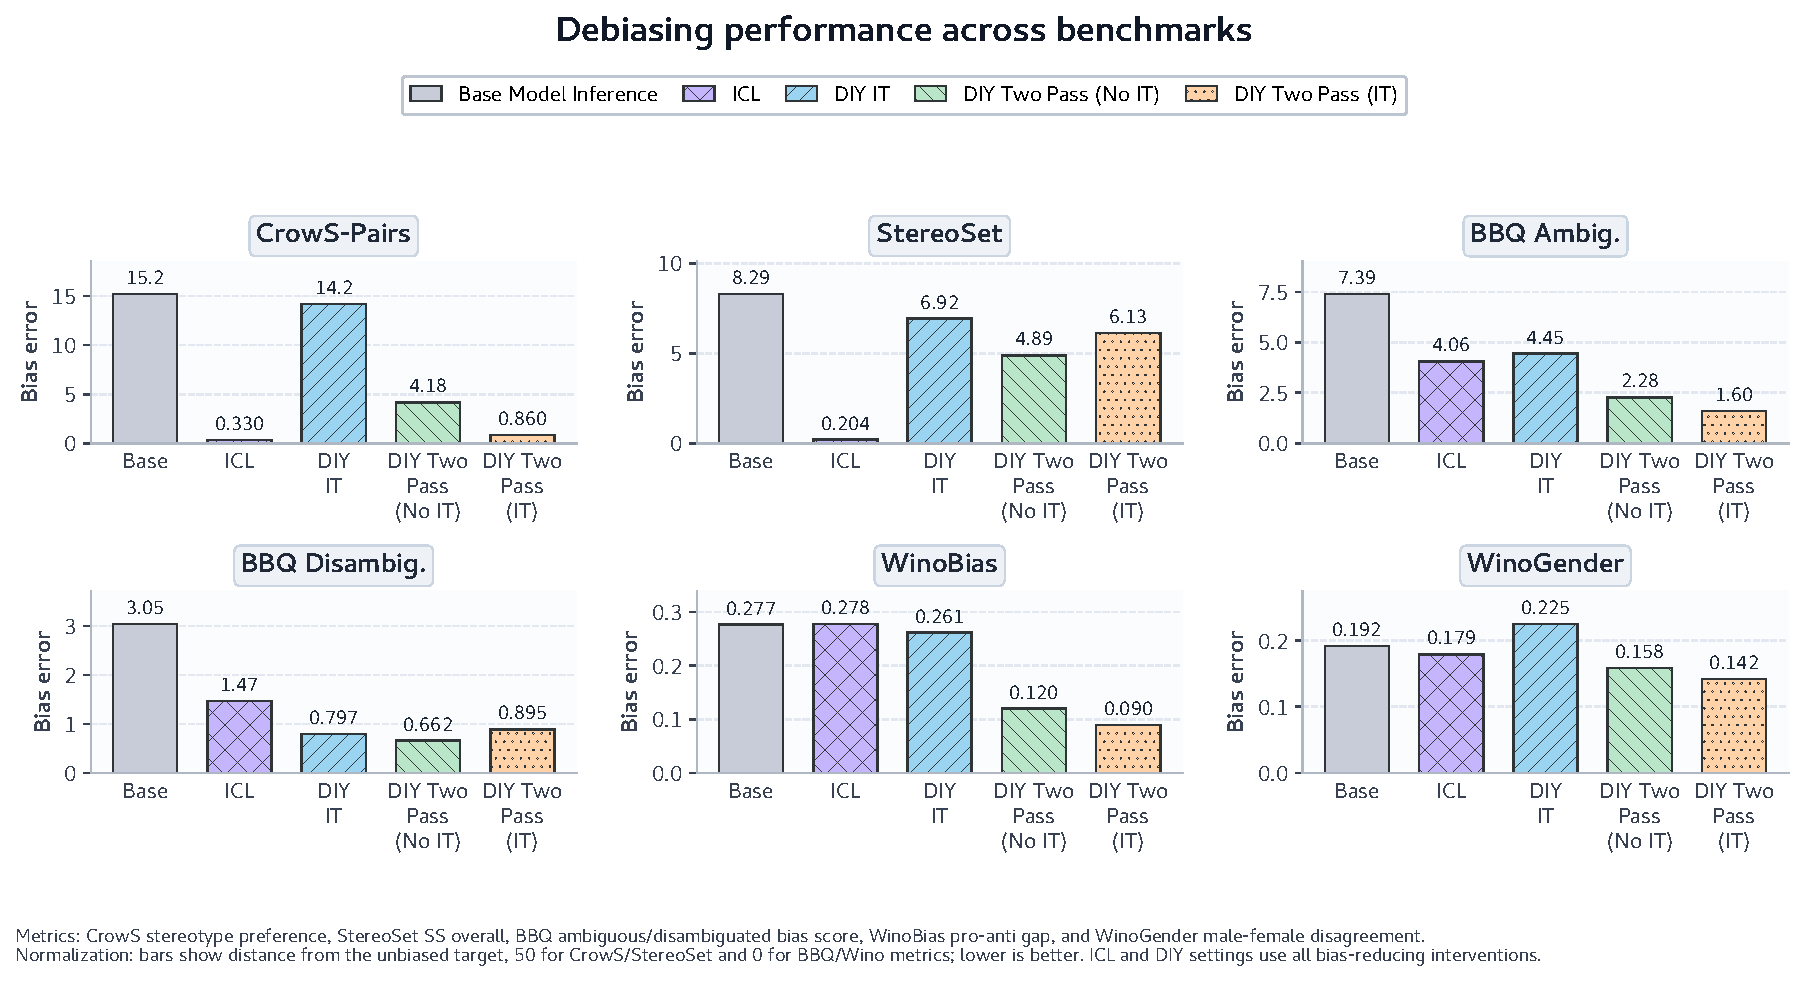
\includegraphics[width=\textwidth]{../../figures/llama8b/pdf/debiasing_method_bars.pdf}
\caption[Debiasing performance of the base model, ICL, and DIY variants]{Debiasing performance of \baseinfer{}, \icllabel{}, and \diy{} variants across the five primary bias benchmarks. Bars report benchmark-native metrics converted to bias error: CrowS-Pairs stereotype preference and StereoSet SS overall are measured as distance from $50$, while BBQ ambiguous/disambiguated bias scores, WinoBias pro--anti gap, and WinoGender male--female pair disagreement are measured as distance from $0$. Lower is better.}
\label{fig:debiasing-method-bars}
\end{figure*}

Figure~\ref{fig:debiasing-method-bars} shows that \diy{} improves the average normalized bias error over \baseinfer{}, with the strongest aggregate reductions coming from inference-time intervention use. Across the six plotted bias metrics, \baseinfer{} has a mean bias error of $5.73$. \icllabel{} reduces this to $1.09$, \diyit{} to $4.47$, \diynoit{} to $2.05$, and \diytpit{} to $1.62$. The pattern is not uniform across datasets, which is important: different benchmarks reward different behaviors, and \diy{}'s gains are clearest when the model can explicitly condition on an intervention-guided procedure.

\begin{table*}[t]
\centering
\small
\setlength{\tabcolsep}{5pt}
\renewcommand{\arraystretch}{1.08}
\begin{tabular}{llcc}
\toprule
Model & Method & Mean bias error $\downarrow$ & Mean reasoning accuracy $\uparrow$ \\
\midrule
\llama{} 8B & \baseinfer{} & 5.73 & 71.95 \\
\llama{} 8B & \icllabel{} & 1.09 & 70.21 \\
\llama{} 8B & \diyit{} & 4.47 & 70.81 \\
\llama{} 8B & \diynoit{} & 2.05 & 74.83 \\
\llama{} 8B & \diytpit{} & 1.62 & 71.24 \\
\midrule
\qwen{} & \baseinfer{} & 4.64 & 87.27 \\
\qwen{} & \icllabel{} & 5.24 & 90.41 \\
\qwen{} & \diyit{} & 4.57 & 92.39 \\
\qwen{} & \diynoit{} & 1.17 & 87.68 \\
\qwen{} & \diytpit{} & 1.77 & 92.96 \\
\midrule
\llama{} 70B & \baseinfer{} & 5.63 & 90.72 \\
\llama{} 70B & \icllabel{} & 2.71 & 89.34 \\
\llama{} 70B & \diyit{} & 5.85 & 89.98 \\
\llama{} 70B & \diynoit{} & 2.08 & 89.84 \\
\llama{} 70B & \diytpit{} & 2.74 & 91.16 \\
\bottomrule
\end{tabular}
\caption{Current aggregate summary across model families. Mean bias error averages the six normalized bias panels used in Figure~\ref{fig:debiasing-method-bars}; mean reasoning accuracy averages ARC-Challenge, ARC-Easy, and Balanced COPA. This table is intended as a compact navigation aid for the current draft rather than a replacement for per-dataset figures.}
\label{tab:aggregate-summary}
\end{table*}

\begin{takeawaybox}
\textbf{Result 1:} \diy{} reduces cross-benchmark bias error relative to \baseinfer{}, with the strongest overall performance from \icllabel{} and \diytpit{}.
\end{takeawaybox}

\subsection{Beating baselines}
\label{sec:results-baselines}

Next, we compare \diy{} against existing mitigation baselines. This comparison is intentionally broad: the baselines include prompting, data-centric, fine-tuning, preference-optimization, and representation-oriented approaches. The purpose is to test whether \diy{} is competitive as a debiasing method, not merely better than the unmitigated base model.

\begin{figure*}[t]
\centering
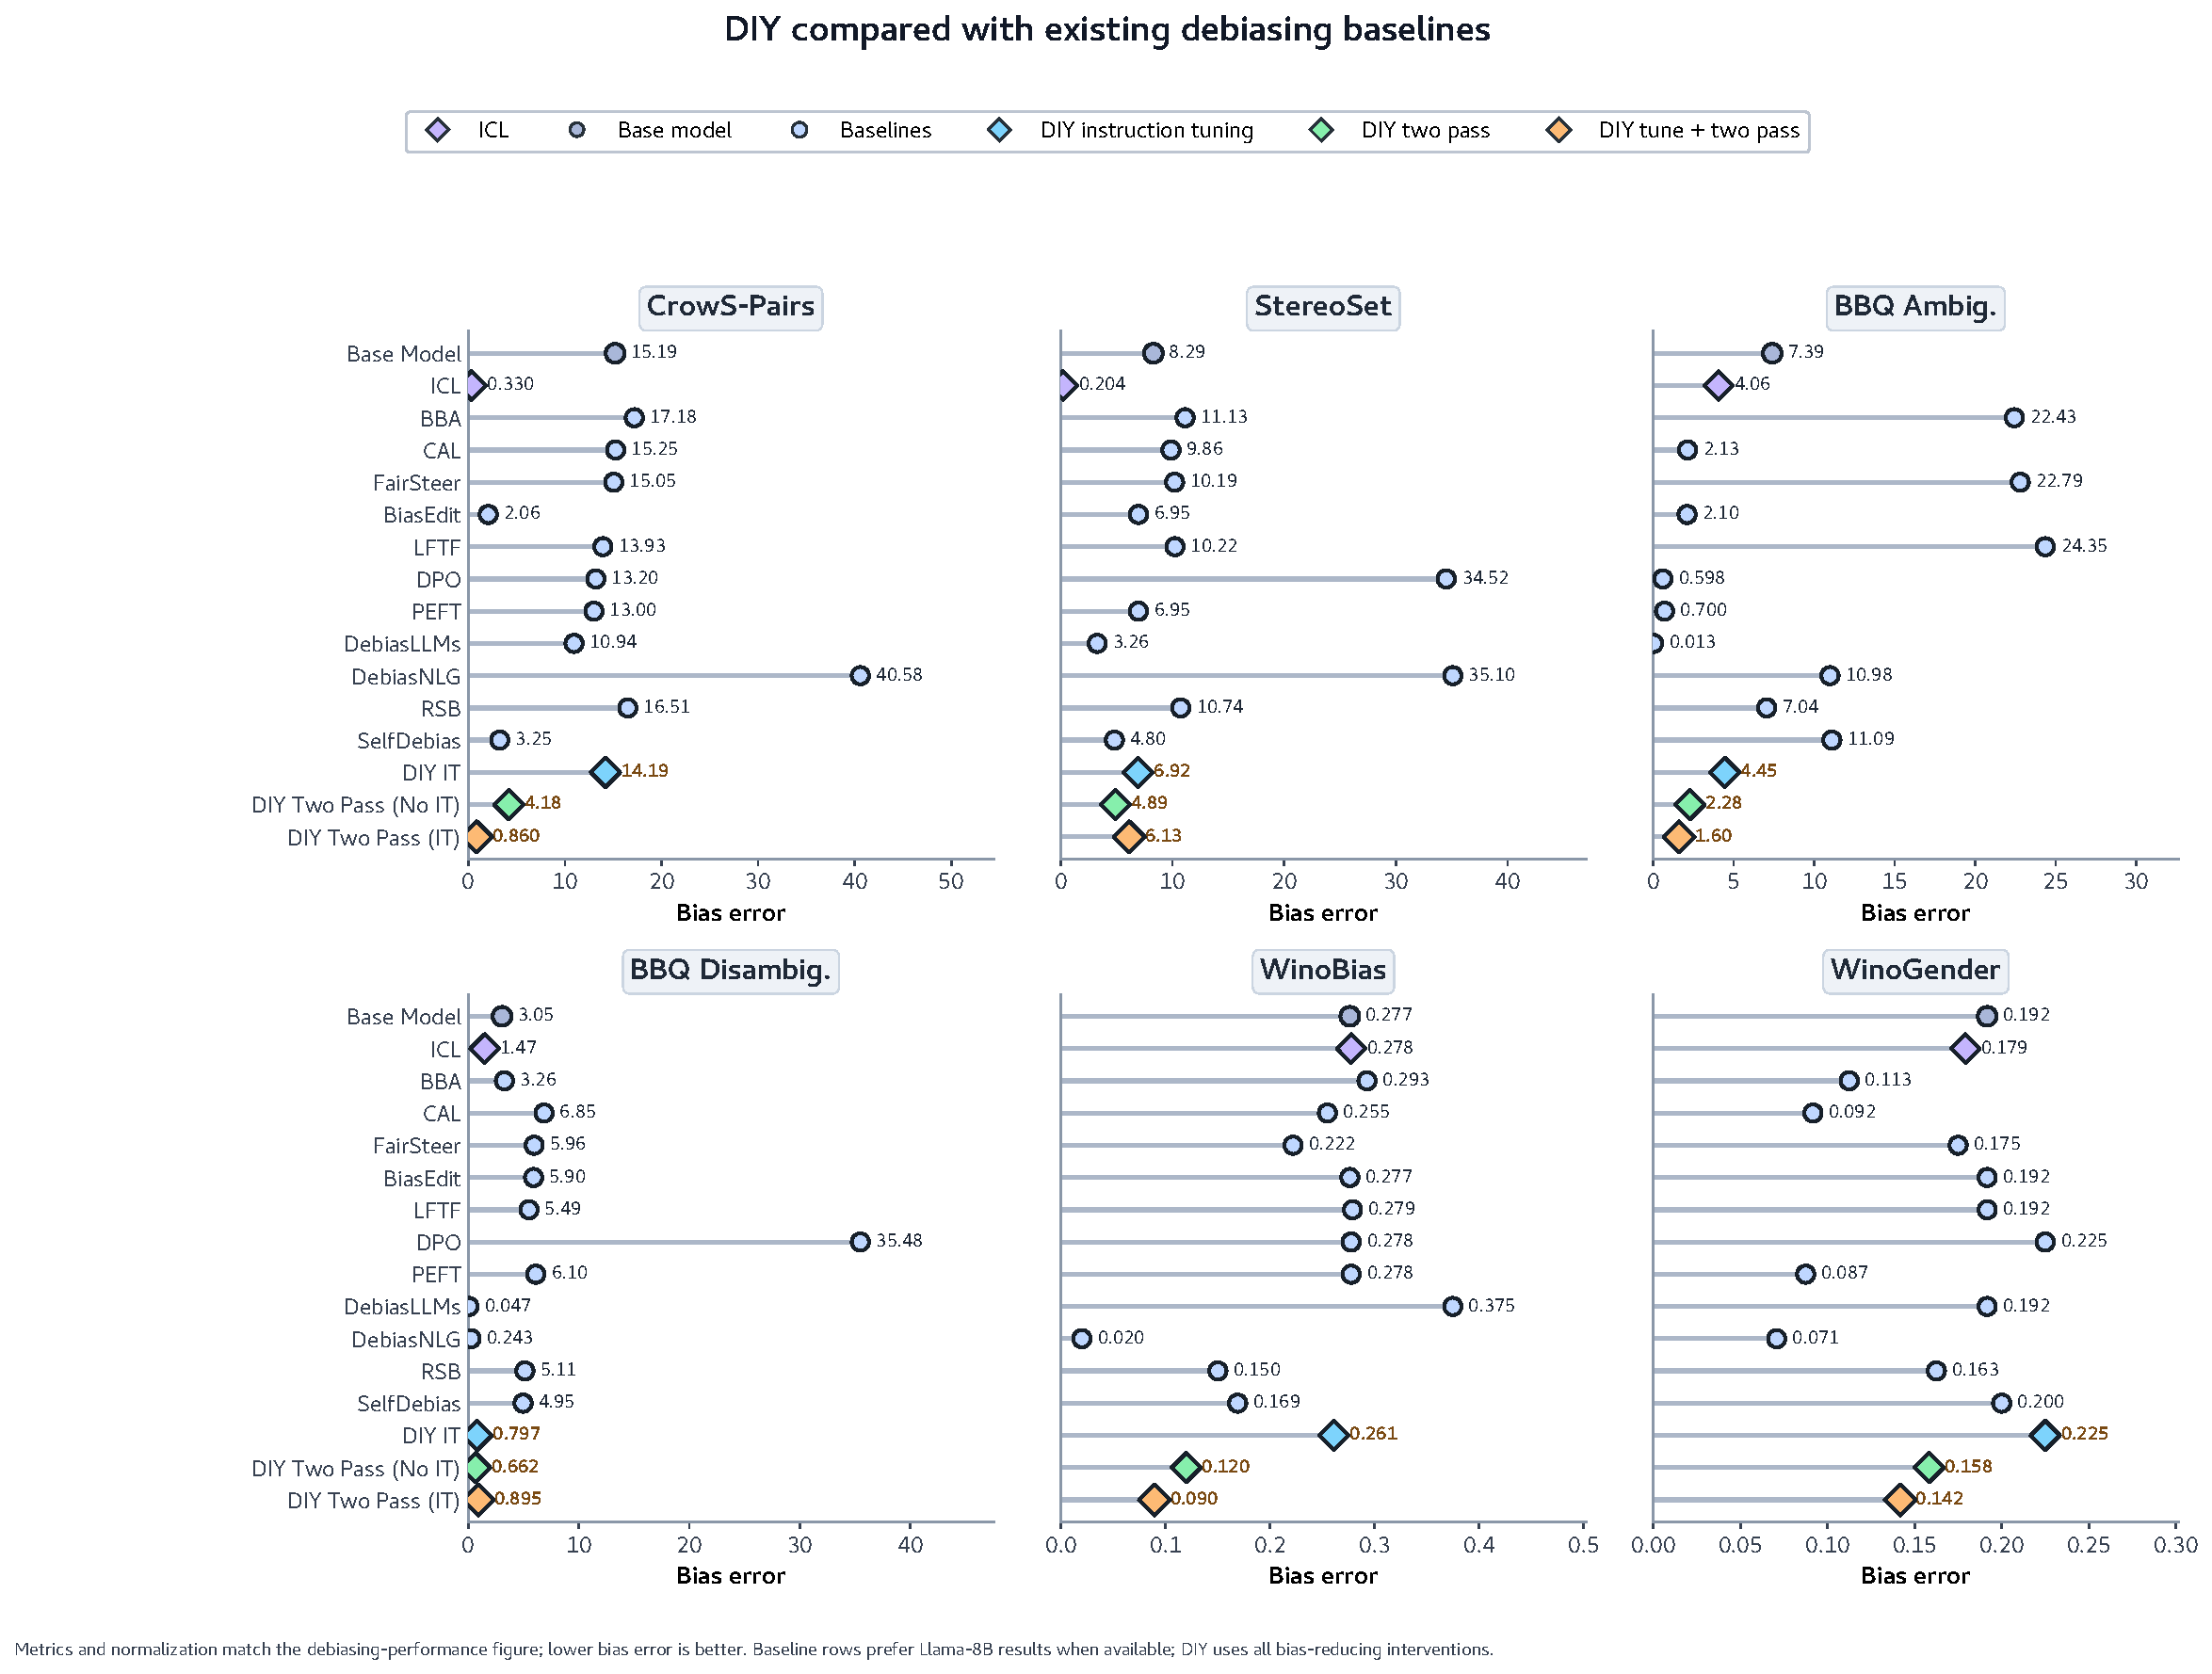
\includegraphics[width=\textwidth]{../../figures/llama8b/pdf/baseline_comparison_lollipop.pdf}
\caption[Comparison between DIY and existing debiasing baselines]{Comparison between \diy{} and existing debiasing baselines. Each lollipop reports the same normalized bias-error metric used in Figure~\ref{fig:debiasing-method-bars}; lower is better. Circles denote \baseinfer{} and prior baselines, while diamonds denote \diy{} variants.}
\label{fig:baseline-comparison}
\end{figure*}

\begin{figure*}[t]
\centering
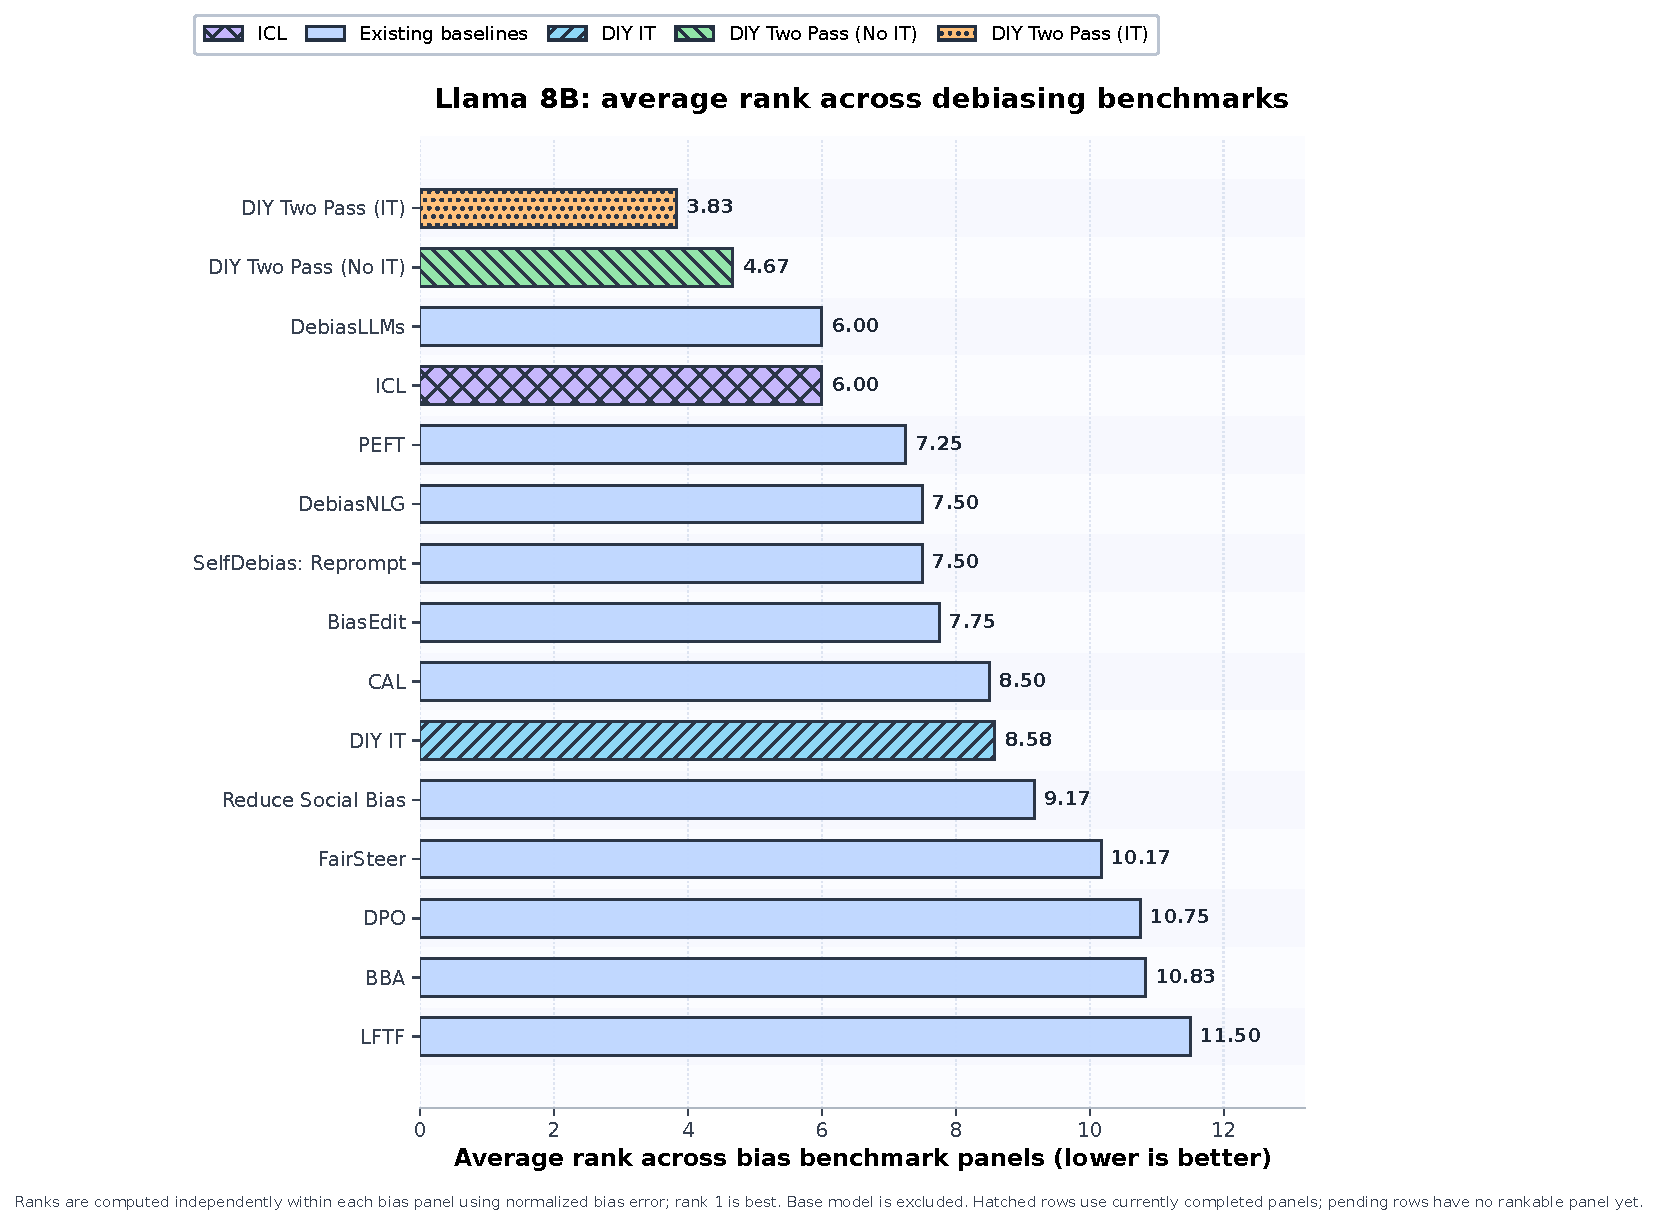
\includegraphics[width=\textwidth]{../../figures/llama8b/pdf/baseline_comparison_average_rank.pdf}
\caption{Average rank of \diy{} and baseline methods across the available bias metrics. Lower rank is better. Ranking complements the lollipop comparison by reducing sensitivity to the scale of any one benchmark metric.}
\label{fig:baseline-rank}
\end{figure*}

Figures~\ref{fig:baseline-comparison} and~\ref{fig:baseline-rank} show that no prior baseline dominates all datasets. Some baselines are strong on individual metrics, but their behavior varies substantially across benchmark families. \diy{} is competitive across this heterogeneous evaluation surface, and \diynoit{} and \diytpit{} are especially strong on both mean bias-error and average-rank comparisons. This supports our framing of \diy{} as structured debiasing supervision rather than as a benchmark-specific patch: the method remains competitive across pairwise likelihood, question answering, and coreference-style evaluations.

\begin{takeawaybox}
\textbf{Result 2:} \diy{} is competitive with a broad set of existing debiasing baselines and is strongest when structured supervision is paired with intervention-guided inference.
\end{takeawaybox}

\subsection{Generalizability}
\label{sec:results-generalizability}

We use interface robustness as one form of generalization: if \diy{} is a reusable debiasing behavior, it should remain useful when the model receives the intervention signal through different inference-time contexts. We therefore compare the main instruction-tuned model with two-pass variants using $0$, $1$, and $2$ demonstrations.

\begin{figure*}[t]
\centering
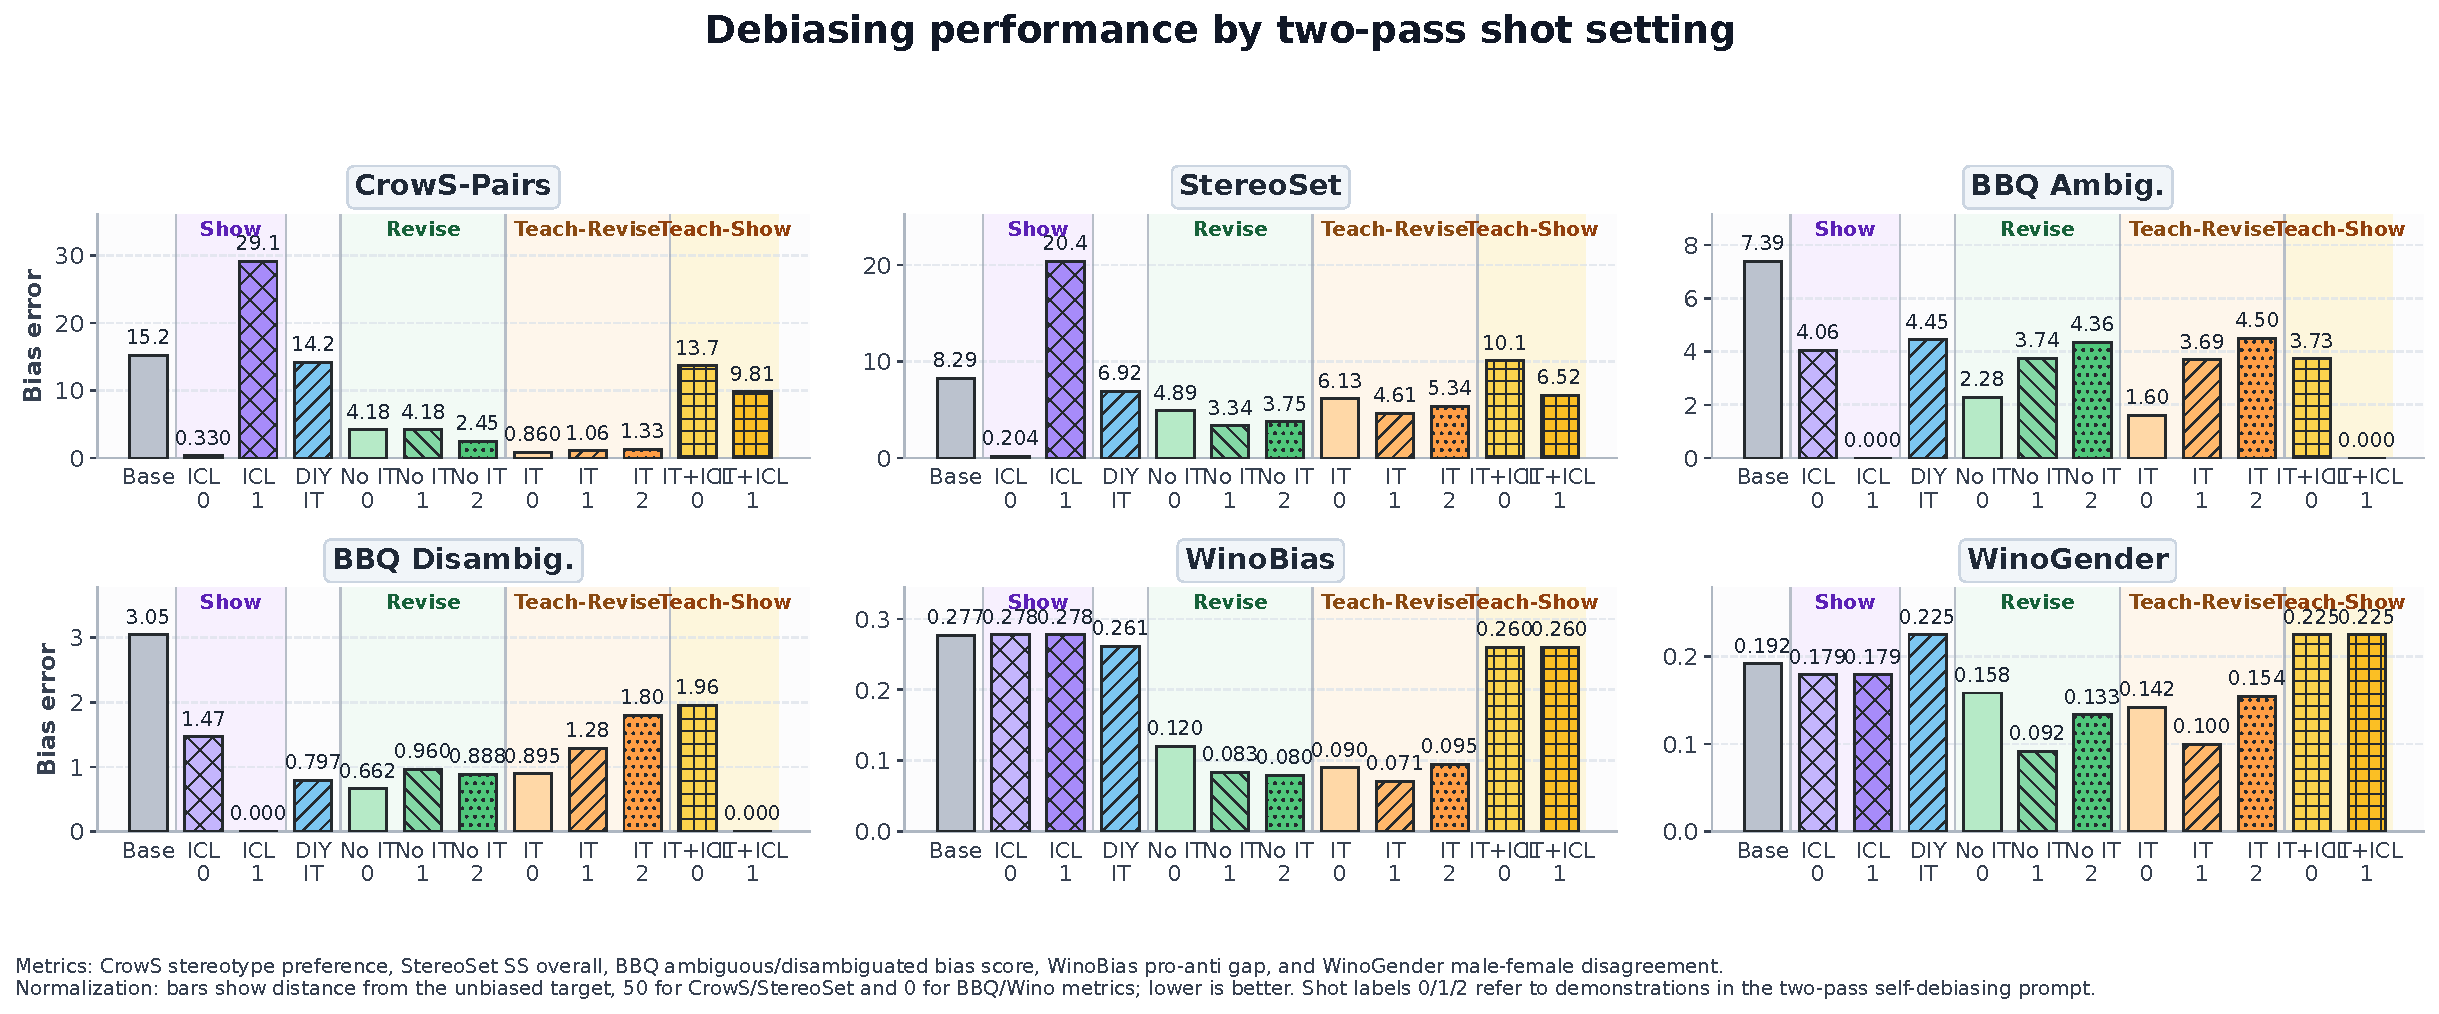
\includegraphics[width=\textwidth]{../../figures/llama8b/pdf/debiasing_method_bars_by_shot.pdf}
\caption[Debiasing performance split by two-pass shot setting]{Debiasing performance split by two-pass shot setting. \baseinfer{} and \diyit{} are shown alongside \diynoit{} and \diytpit{} with $0$, $1$, and $2$ demonstrations. Metrics and normalization match Figure~\ref{fig:debiasing-method-bars}; lower is better.}
\label{fig:debiasing-by-shot}
\end{figure*}

Figure~\ref{fig:debiasing-by-shot} shows that \diy{} is not tied to a single delivery mechanism. \diyit{} provides a learned interface to intervention-labeled supervision, while \diynoit{} and \diytpit{} activate the same intervention inventory at inference time. The shot-level comparison also reveals that additional demonstrations are not uniformly beneficial: some datasets improve with more demonstrations, while others are best under zero-shot inference. This suggests that the intervention signal itself is useful, but benchmark format and prompt sensitivity still matter.

\begin{takeawaybox}
\textbf{Result 3:} \diy{} generalizes across training-time and inference-time interfaces, but the best shot setting depends on the benchmark and metric.
\end{takeawaybox}

\subsection{Bias vs. utility/reasoning}
\label{sec:results-utility}

A debiasing method is not useful if it reduces bias by becoming evasive, invalid, or generally less competent. We therefore evaluate the same main variants on ARC-Challenge, ARC-Easy, and Balanced COPA, and then compare methods by their bias--utility tradeoff.

\begin{figure*}[t]
\centering
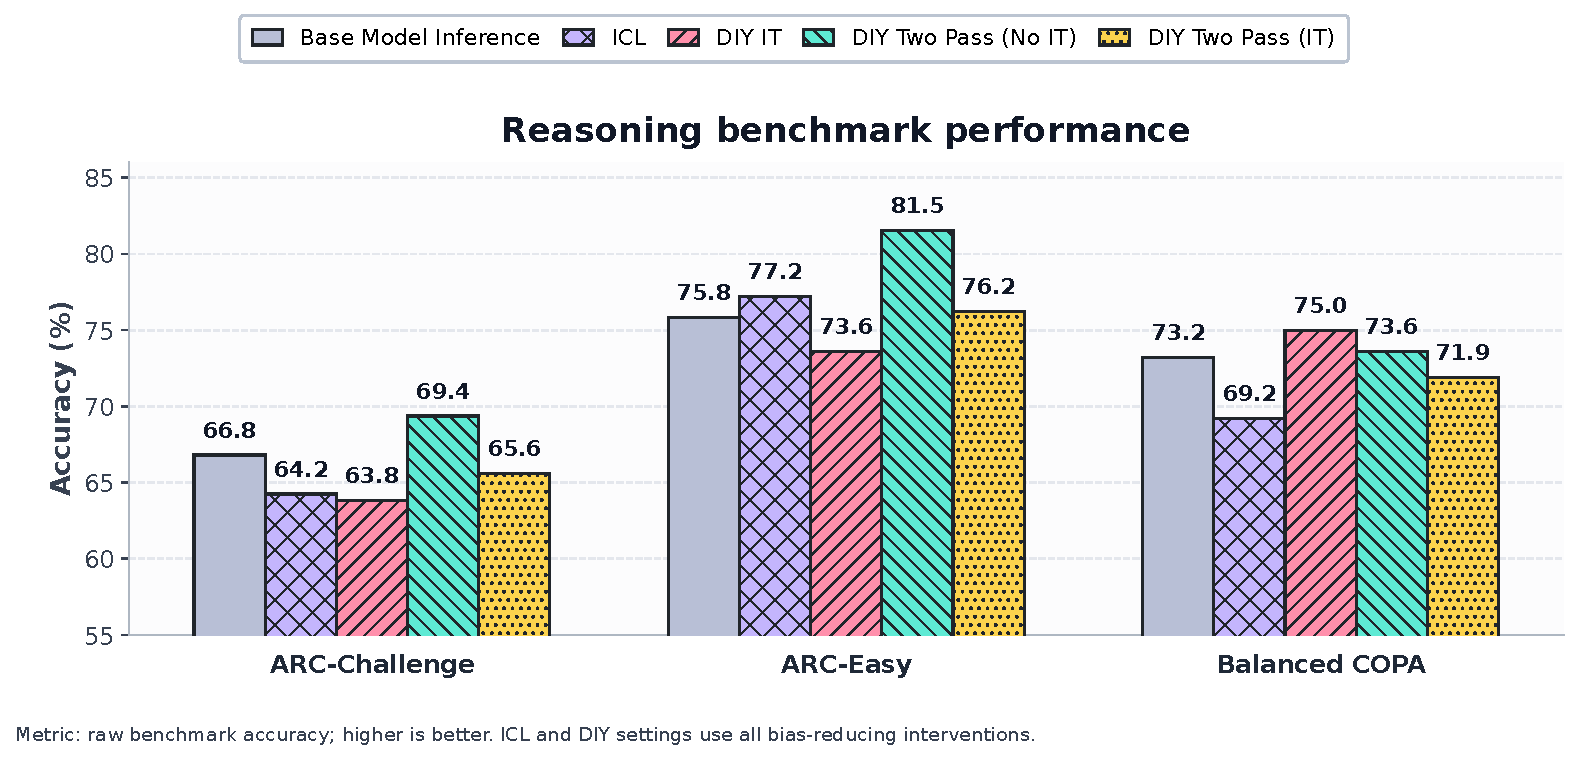
\includegraphics[width=\textwidth]{../../figures/llama8b/pdf/reasoning_performance.pdf}
\caption[Reasoning benchmark performance for the base model and DIY variants]{Reasoning benchmark performance for \baseinfer{} and \diy{} variants. Scores are raw accuracy on ARC-Challenge, ARC-Easy, and Balanced COPA; higher is better.}
\label{fig:reasoning-performance}
\end{figure*}

\begin{figure*}[t]
\centering
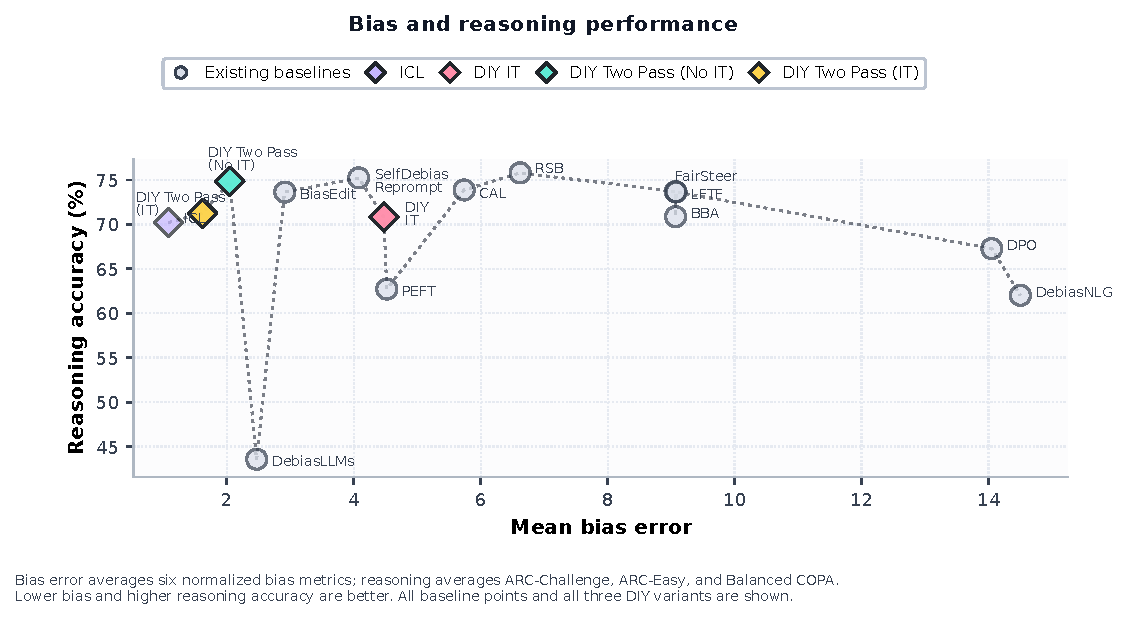
\includegraphics[width=\textwidth]{../../figures/llama8b/pdf/bias_reasoning_pareto.pdf}
\caption{Bias--utility tradeoff across baselines and \diy{} variants. The $x$-axis is mean normalized bias error over the six bias panels; the $y$-axis is mean reasoning accuracy over ARC-Challenge, ARC-Easy, and Balanced COPA. Lower-left to upper-left movement indicates better bias mitigation without sacrificing reasoning.}
\label{fig:bias-reasoning-pareto}
\end{figure*}

Figure~\ref{fig:reasoning-performance} shows that \diynoit{} and \diytpit{} preserve or improve reasoning accuracy in several settings, especially for ARC-Easy and Balanced COPA. \diyit{} alone is more mixed on ARC, which suggests that structured debiasing supervision is not automatically utility-neutral. \icllabel{} is also useful as a control: it can reduce bias strongly, but its reasoning behavior depends on benchmark format. Figure~\ref{fig:bias-reasoning-pareto} summarizes the overall tradeoff: methods vary not only in bias reduction but also in reasoning preservation. The desired region is low bias error with high reasoning accuracy; \diy{} variants move toward this region more consistently than methods that reduce bias by degrading task performance.

\begin{takeawaybox}
\textbf{Result 4:} \diy{} can reduce bias while preserving reasoning, but the tradeoff depends on the interface; \diynoit{} and \diytpit{} give the strongest bias--utility profile in the current results.
\end{takeawaybox}

\subsection{Ablations}
\label{sec:results-ablations}

Finally, we test whether the five bias-reducing interventions matter. If \diy{} were only generic debiasing data, then intervention-specific variants should behave similarly. Instead, we expect different interventions to specialize across task formats, with the all-intervention framing providing a robust aggregate method.

\begin{figure*}[t]
\centering
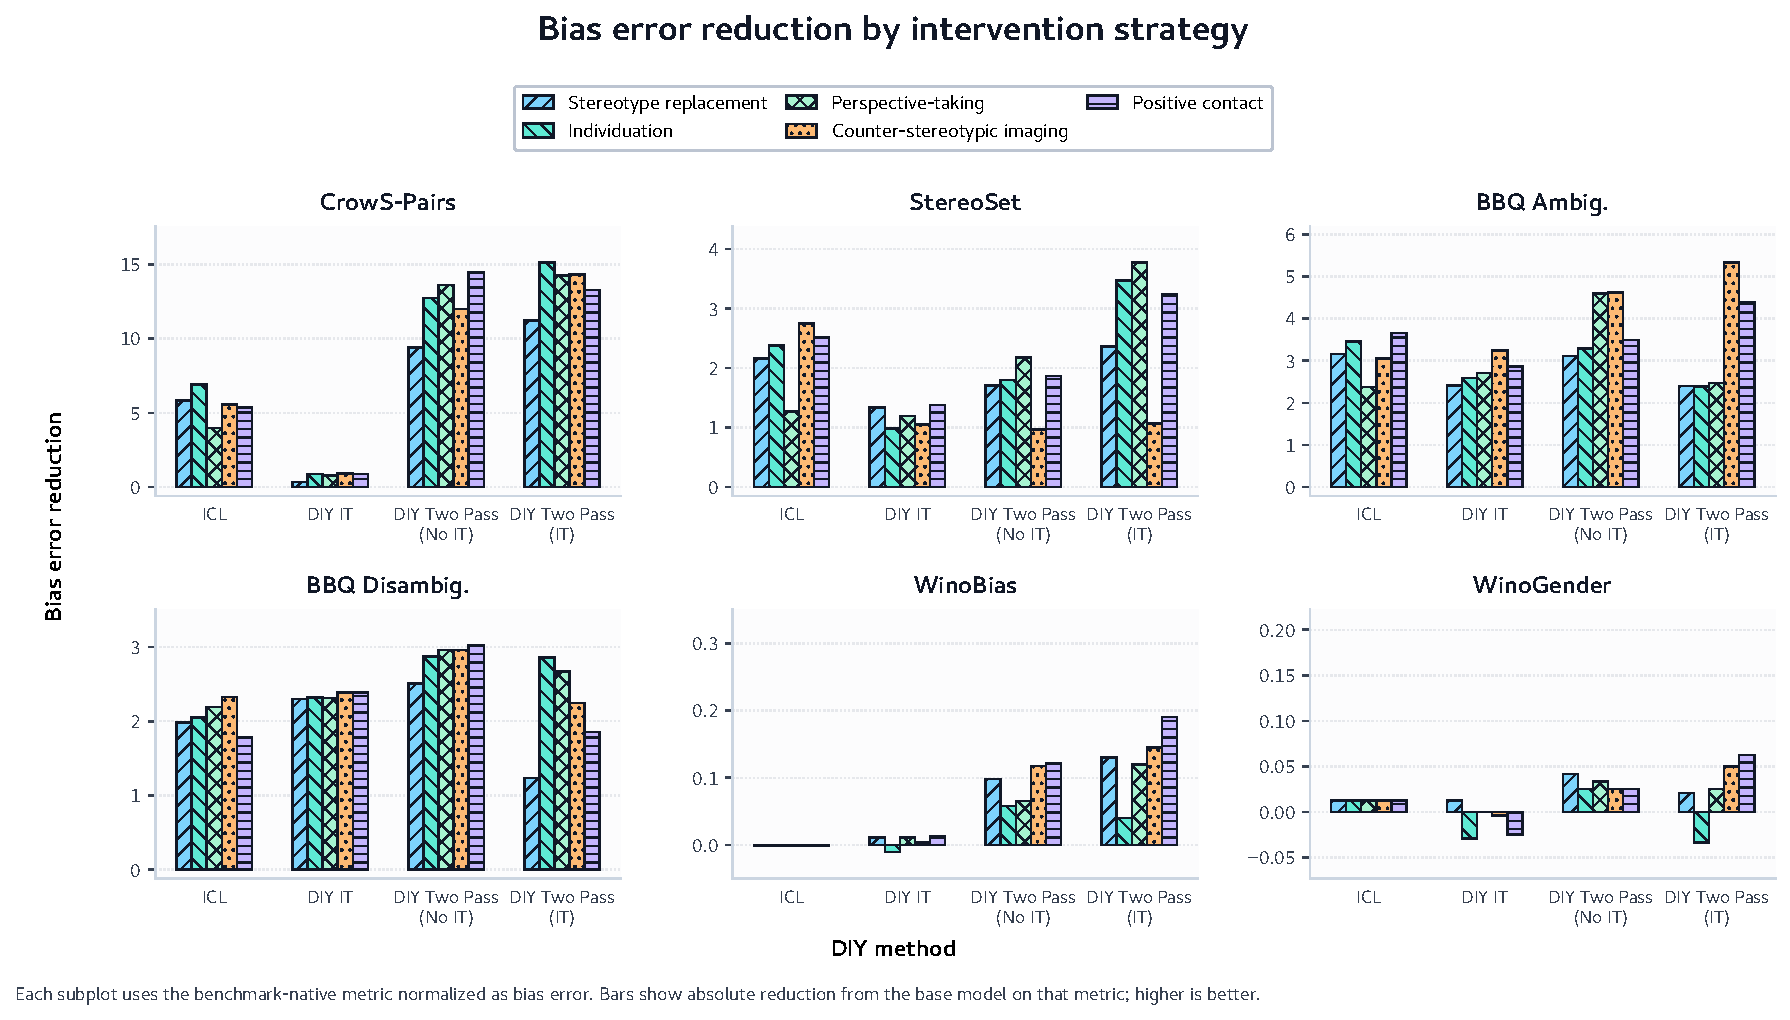
\includegraphics[width=\textwidth]{../../figures/llama8b/pdf/intervention_ablation.pdf}
\caption[Intervention ablation across DIY variants]{Intervention ablation across \diy{} variants. Bars report bias-error reduction relative to \baseinfer{} for each benchmark panel; higher is better. Colors correspond to \srfull{}, \indfull{}, \ptfull{}, \cifull{}, and \pcfull{}.}
\label{fig:intervention-ablation}
\end{figure*}

Figure~\ref{fig:intervention-ablation} shows that intervention choice changes behavior. No single intervention is uniformly best across all datasets and interfaces. \ptfull{} and \pcfull{} are strong in several two-pass settings, while \indfull{} is especially useful when the task rewards attention to instance-specific evidence. \diyit{} has smaller but consistent gains across interventions. These patterns support the central design choice of \diy{}: debiasing supervision should expose multiple reusable bias-reducing behaviors rather than force all examples through one generic instruction.

We include companion \qwen{} and \llama{}-70B plots in Appendix~\ref{sec:appendix-model-results}. These plots do not replace the \llama{} 8B main results because the auxiliary and fine-grained matrices are incomplete in different ways, but the main debiasing and reasoning summaries now cover the same five method families. They are useful sanity checks because they expose where the \diy{} interface appears model-sensitive.

\begin{takeawaybox}
\textbf{Result 5:} The intervention inventory is not decorative; \srfull{}, \cifull{}, \indfull{}, \ptfull{}, and \pcfull{} specialize across benchmarks, and their mixture supports broader mitigation.
\end{takeawaybox}

\FloatBarrier

\section{Analysis}
\label{sec:analysis}

\subsection{What Does ``Generalizable'' Mean Here?}
\label{sec:generalization}

We define generalization along four axes. \textbf{Identity generalization} means the method is not tuned only to gender or race but applies across age, disability, nationality, religion, sexuality, socioeconomic status, and other axes. \textbf{Task generalization} means transfer across likelihood ranking, question answering, generation, and coreference-style evaluation. \textbf{Domain generalization} means improvement across benchmarks collected under different assumptions and annotation procedures. \textbf{Interface generalization} means that the same intervention-labeled supervision remains useful when instantiated through training-time and inference-time mechanisms.

The current evidence should be presented as partial generalization, not complete generalization. \diy{} tests a broader surface than many single-benchmark mitigation methods, but all evaluations are still benchmark-mediated and English-centered. The final paper should report where transfer fails as prominently as where it succeeds.

\subsection{Why These Interventions?}
\label{sec:why-psych}

The value of the socio-psychological source is not anthropomorphism. We do not argue that models have prejudice habits. Rather, prejudice-reducing interventions give us a compact design space for debiasing supervision. \srfull{} teaches explicit rejection and substitution. \indfull{} teaches evidence use. \ptfull{} teaches impact-aware inference. \cifull{} and \pcfull{} teach distributional diversification. Together, they define a structured supervision signal that is more precise than an ad hoc instruction such as ``do not be biased.''

\subsection{Failure Modes}
\label{sec:failure-modes}

We expect four recurring failure modes.
First, some conditioned outputs may produce generic safety language rather than solving the task. Second, likelihood-based benchmarks can be distorted by verbose rationale text. Third, generated debiasing data can over-sanitize examples and reduce task diversity. Fourth, self-revision can improve bias metrics by changing answer style rather than by improving underlying evidence use. These risks motivate our use of multiple datasets and reasoning checks.

\section{Discussion}
\label{sec:discussion}

\diy{} is best understood as a structured debiasing supervision method with a psychologically motivated intervention inventory. It asks whether models can learn reusable mappings from biased inputs to evidence-grounded outputs, and whether those mappings transfer across bias surfaces. This framing separates the contribution from any single implementation mechanism and creates a more demanding evaluation standard: if the method is generalizable, it should show evidence across identities, benchmarks, and task types.

The strongest paper version should emphasize three results. First, \diy{} produces competitive or strong bias mitigation across several benchmarks relative to existing baselines in the complete \llama{} 8B matrix. Second, the ablations show why the method works: intervention mixtures and structured supervision are more robust than unstructured instructions or single narrow interventions. Third, reasoning preservation is interface- and model-dependent: two-pass inference gives a strong bias--utility profile in the main matrix, and the companion \qwen{} and \llama{}-70B results show that the same interfaces remain competitive across model families, although some auxiliary cells are still missing.

This gives the paper a balanced but assertive claim. The method is not a universal debiasing solution. It is a generalizable structured supervision method that improves over narrower mitigation baselines by teaching models evidence-grounded bias-reducing behaviors.

\section{Conclusion}
\label{sec:conclusion}

We introduced \diy{}, a structured supervision method for generalizable language-model bias mitigation. \diy{} translates prejudice-reducing interventions from social psychology into model-facing bias-reducing interventions, generates intervention-labeled supervision across identity dimensions and instance types, and induces models to replace unsupported social-group heuristics with evidence-grounded outputs. The experimental design evaluates whether this method outperforms narrower debiasing baselines across benchmark formats while preserving reasoning performance. Current results show strong gains in the complete \llama{} 8B matrix and consistent companion evidence from \qwen{} and \llama{}-70B under the available bias and reasoning metrics.

\section*{Limitations}
\label{sec:limitations}

The current paper has several known limitations. First, several citation placeholders need verification before submission. Second, the evaluation is mostly English and benchmark-based, so claims about real-world bias mitigation should remain cautious. Third, generated biased examples can contain harmful stereotypes; the final paper must describe filtering, storage, and release decisions carefully. Fourth, some auxiliary companion-model and fine-grained cells remain incomplete, even though the main debiasing and reasoning plots are now populated for all three model families. Fifth, reasoning preservation is mixed and should not be overstated.

\section*{Ethical Considerations}
\label{sec:ethical}

\diy{} intentionally generates and manipulates biased text in order to train and evaluate mitigation methods. This creates risks: synthetic examples can reproduce harmful stereotypes, benchmark improvements can create false confidence, and identity descriptors can be overgeneralized. We mitigate these risks by using the data for controlled research, evaluating across multiple identity dimensions, and explicitly distinguishing model behavior from human implicit attitudes. The final release plan should avoid publishing harmful generated examples without filtering, documentation, and access controls where appropriate.

\bibliography{anthology,custom}

\appendix
\clearpage
\section{Draft Appendix Checklist}
\label{sec:appendix-checklist}

The final appendix should include:
\begin{itemize}[leftmargin=1.4em,itemsep=1pt,topsep=2pt]
    \item full intervention prompts for all five interventions;
    \item data generation templates and filtering rules;
    \item model and LoRA hyperparameters;
    \item all benchmark metric definitions;
    \item full per-dataset result tables;
    \item per-intervention ablations;
    \item reasoning benchmark details;
    \item safety and data release documentation.
\end{itemize}

\section{Companion Model Results}
\label{sec:appendix-model-results}

The main paper uses the \llama{} 8B matrix for the primary narrative because it has the richest set of baseline, ablation, shot, and CI overlays. We additionally generate companion plots for \qwen{} and \llama{}-70B to inspect whether the same interfaces behave similarly under alternative model families and scales. These figures should be read as diagnostic evidence: the main debiasing and reasoning plots are populated, while some auxiliary and fine-grained cells remain missing and are tracked in \texttt{figures/qwen/csv/} and \texttt{figures/llama70b/csv/}.

\begin{figure*}[t]
\centering
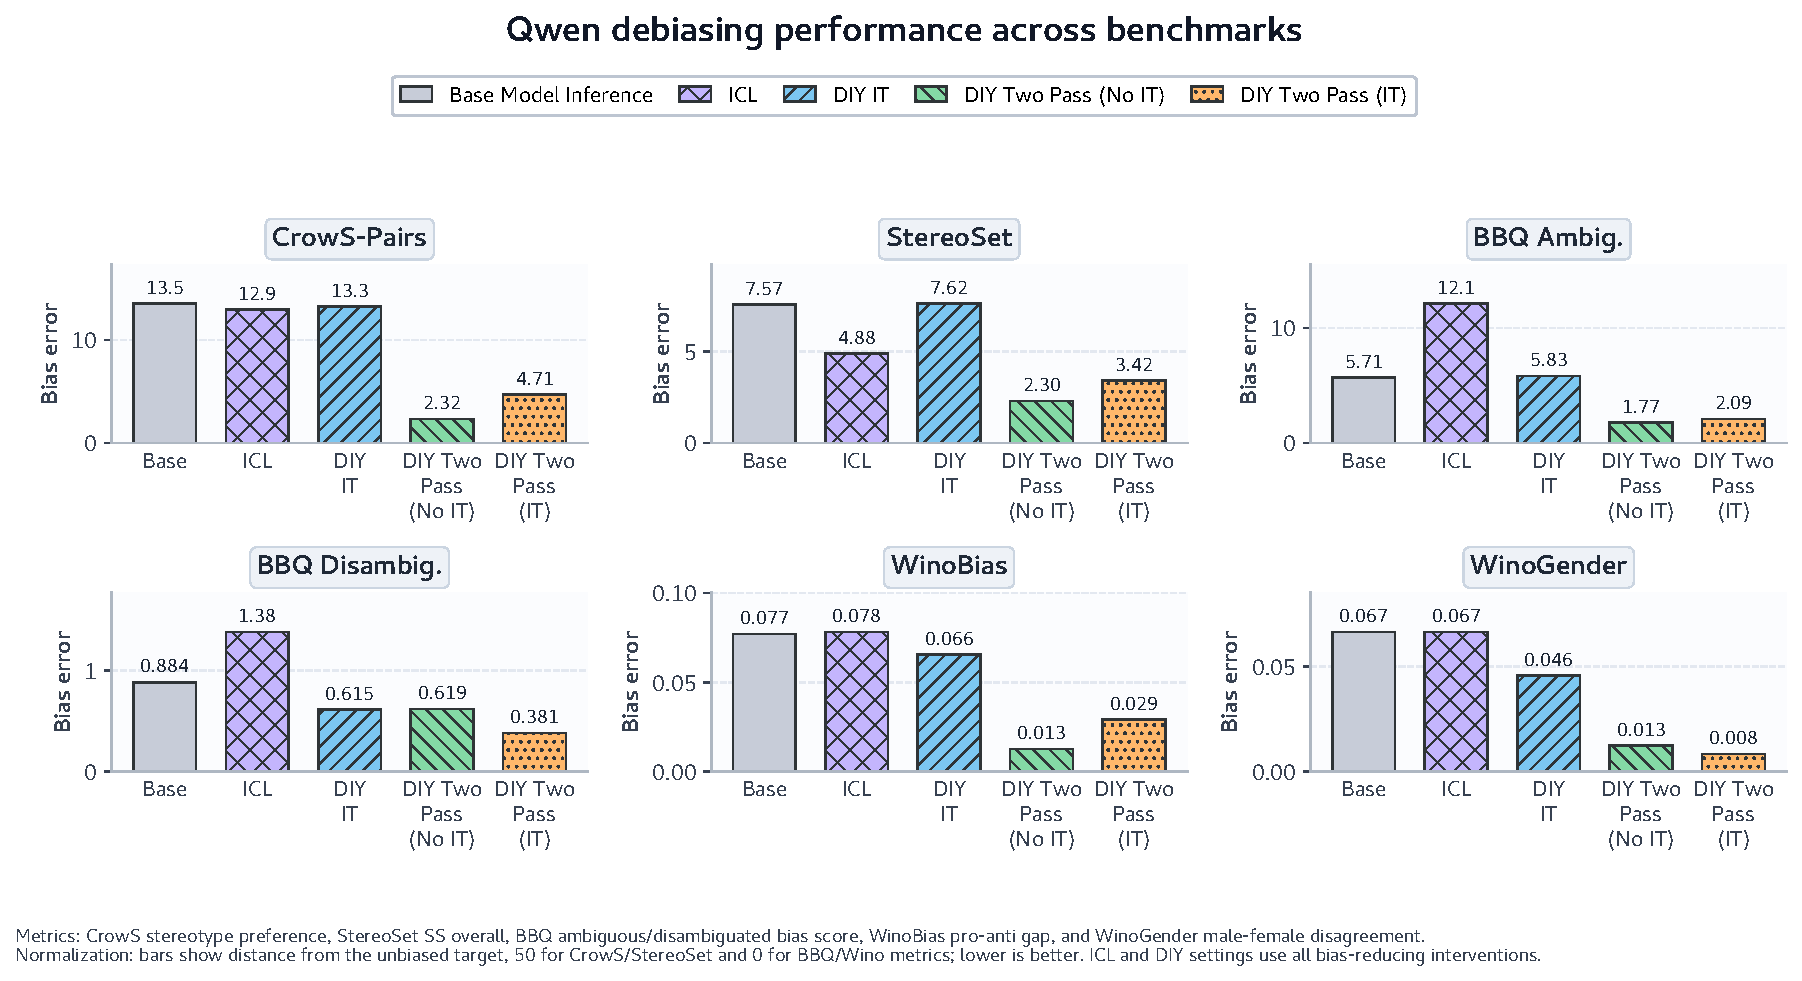
\includegraphics[width=\textwidth]{../../figures/qwen/pdf/debiasing_method_bars.pdf}
\caption[Qwen debiasing performance under the available bias metrics]{\qwen{} debiasing performance under the available bias metrics. The figure uses the same bias-error normalization as Figure~\ref{fig:debiasing-method-bars} and includes \baseinfer{}, \icllabel{}, \diyit{}, \diynoit{}, and \diytpit{}.}
\label{fig:qwen-debiasing}
\end{figure*}

\begin{figure*}[t]
\centering
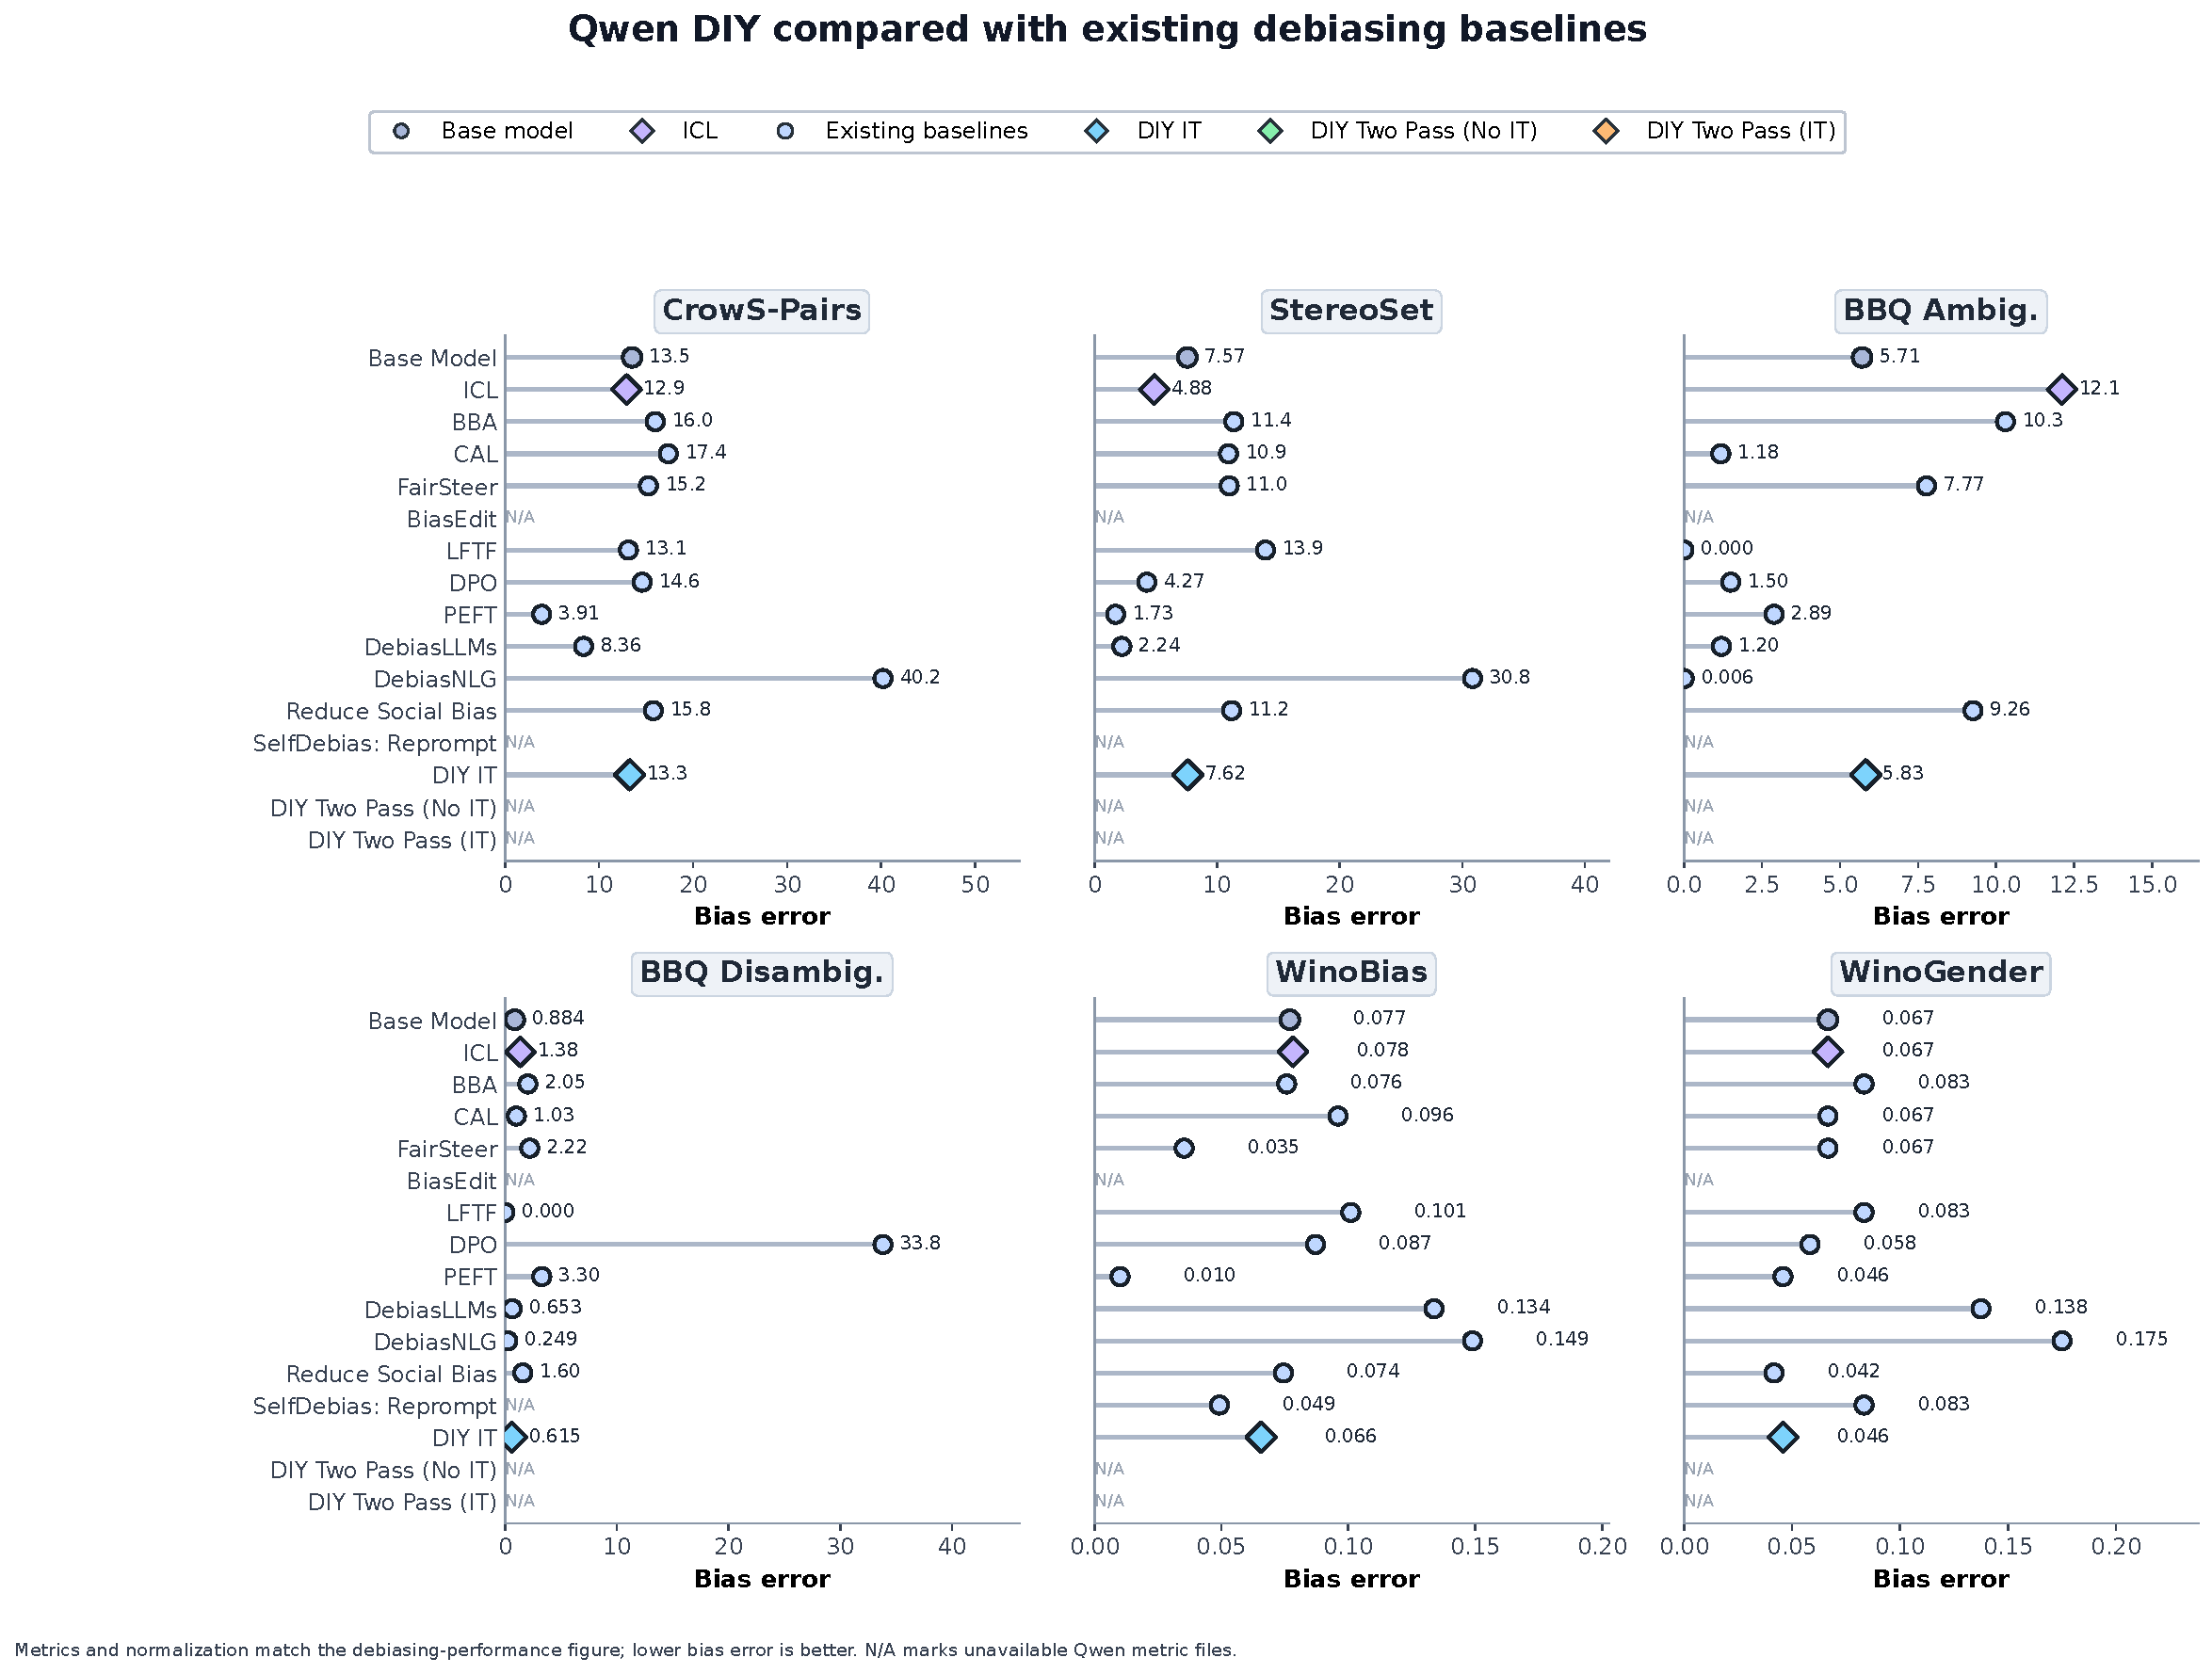
\includegraphics[width=\textwidth]{../../figures/qwen/pdf/baseline_comparison_lollipop.pdf}
\caption{\qwen{} comparison with existing debiasing baselines. Metrics and normalization match the main \llama{} 8B baseline comparison.}
\label{fig:qwen-baselines}
\end{figure*}

\begin{figure*}[t]
\centering
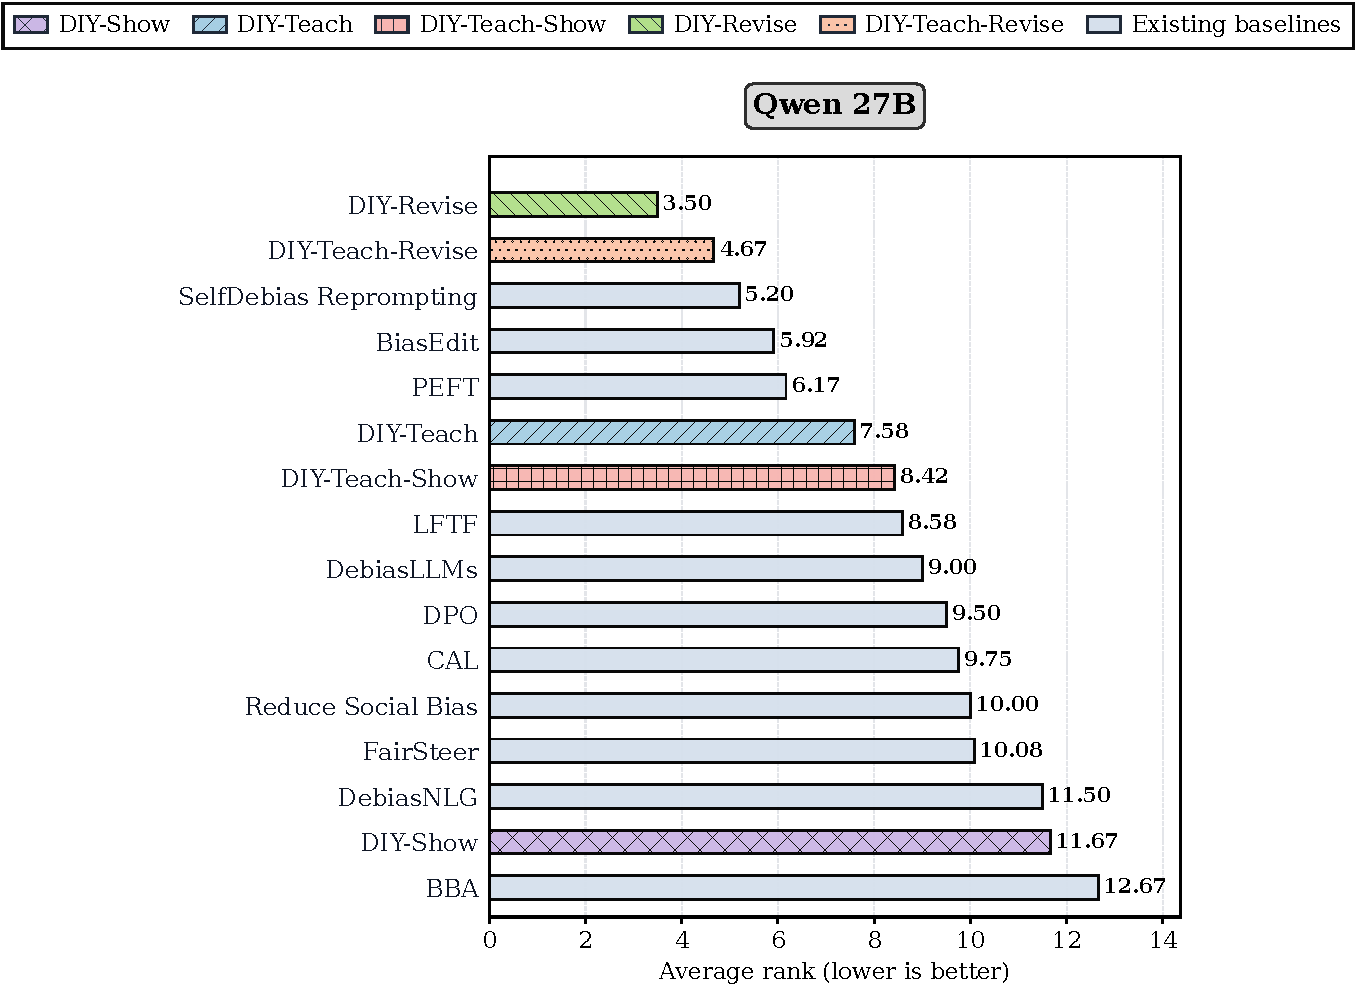
\includegraphics[width=\textwidth]{../../figures/qwen/pdf/baseline_comparison_average_rank.pdf}
\caption{\qwen{} average-rank comparison across the available bias metrics. Lower rank is better.}
\label{fig:qwen-average-rank}
\end{figure*}

\begin{figure*}[t]
\centering
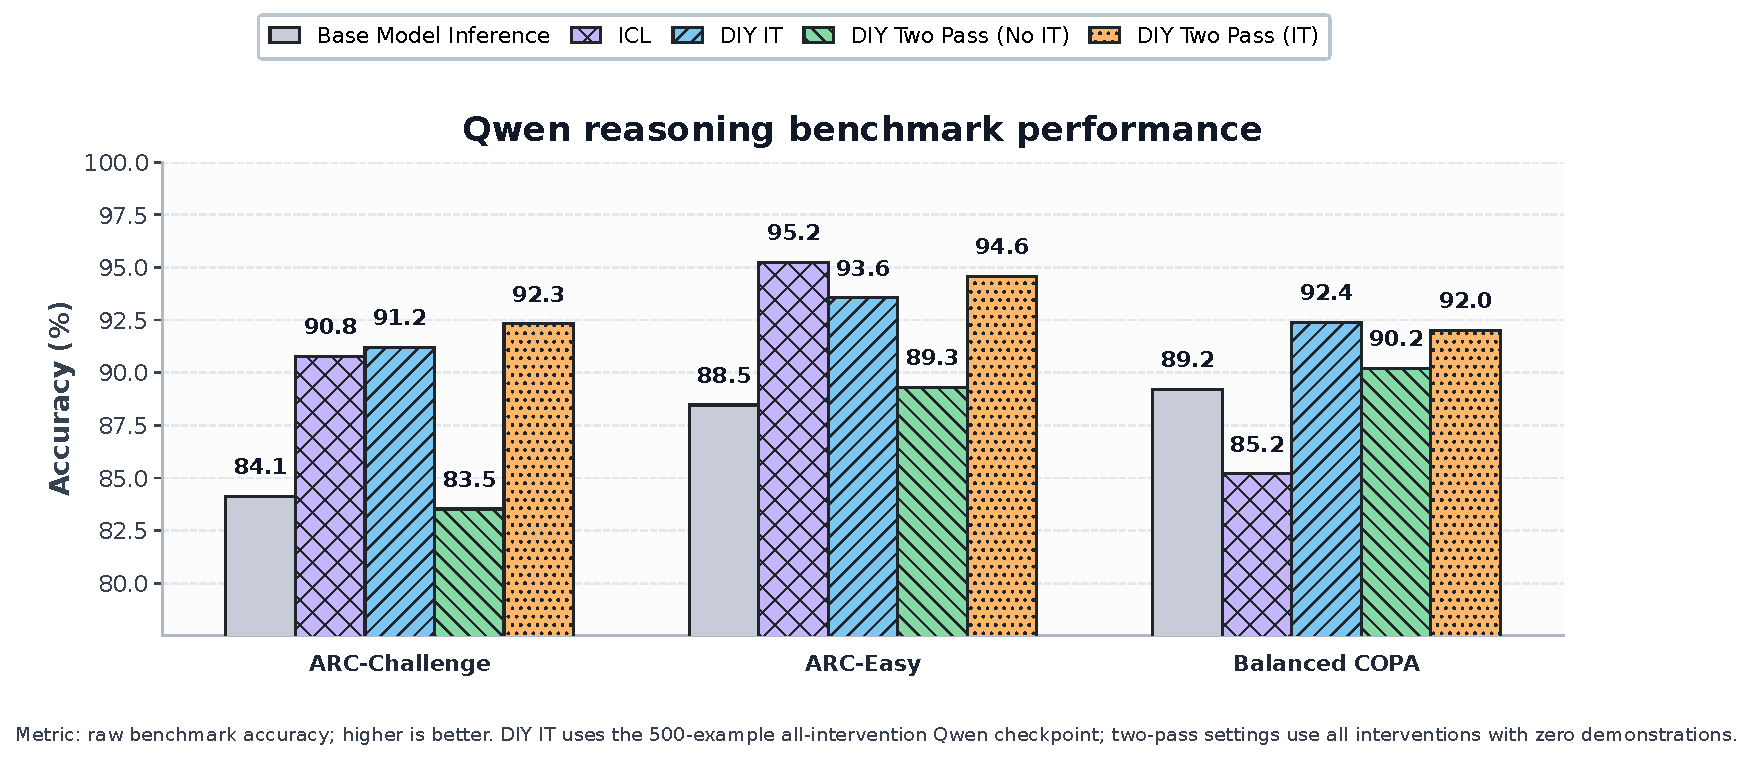
\includegraphics[width=\textwidth]{../../figures/qwen/pdf/reasoning_performance.pdf}
\caption[Qwen reasoning performance for the base model and DIY variants]{\qwen{} reasoning performance for \baseinfer{} and \diy{} variants. The reasoning matrix is complete for the main \baseinfer{}, \diyit{}, \diynoit{}, and \diytpit{} variants.}
\label{fig:qwen-reasoning}
\end{figure*}

\begin{figure*}[t]
\centering
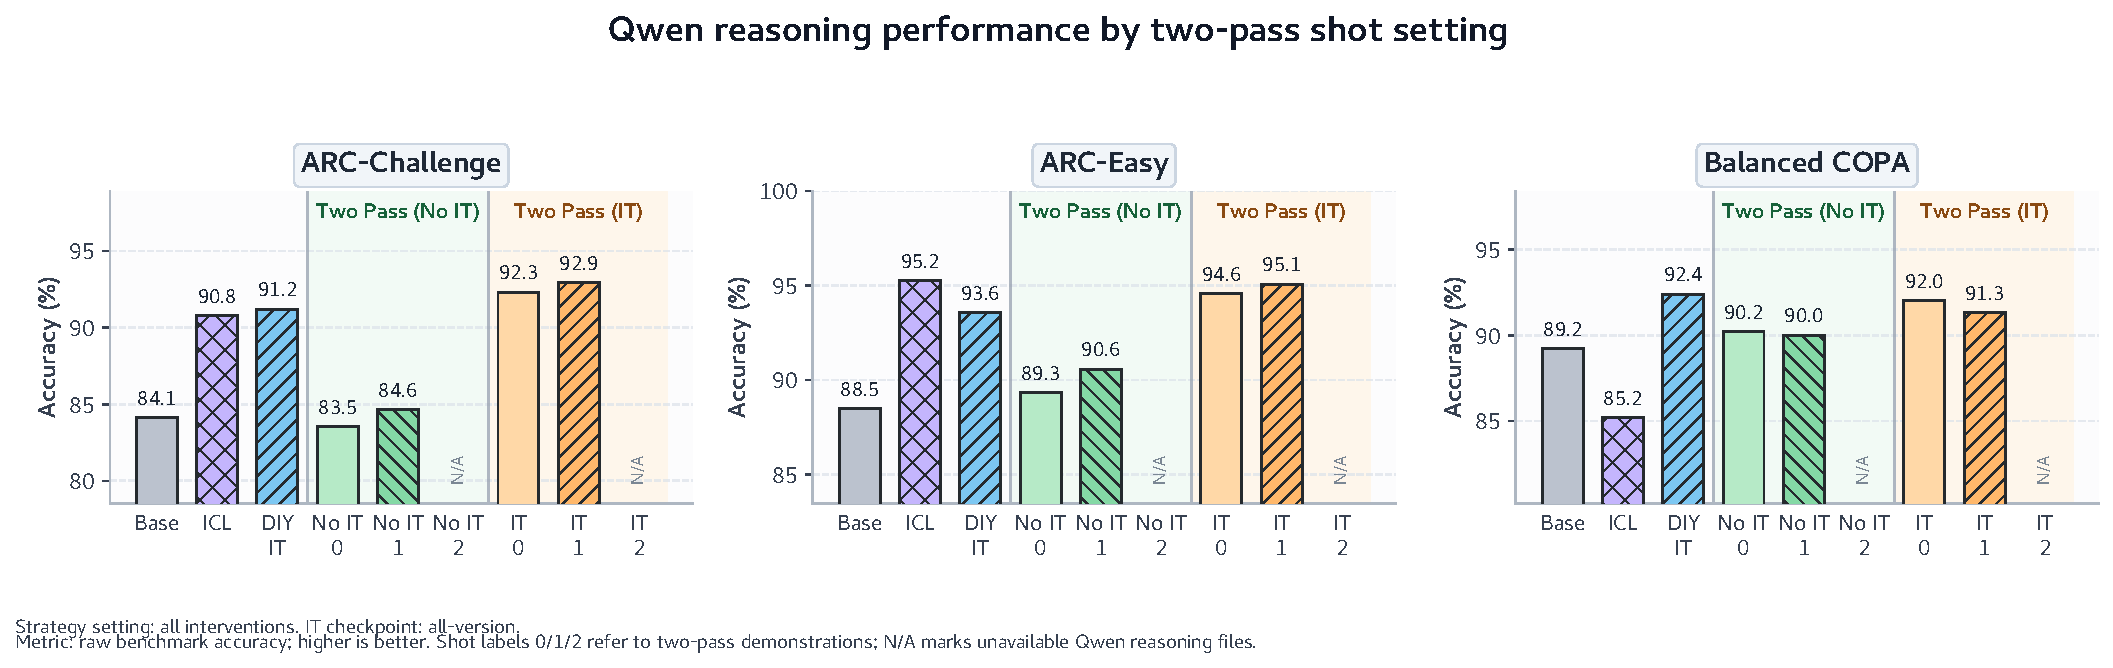
\includegraphics[width=\textwidth]{../../figures/qwen/pdf/reasoning_performance_by_shot.pdf}
\caption{\qwen{} reasoning performance by two-pass shot setting. The added \qwen{} results primarily expand this reasoning analysis, showing how zero-, one-, and two-demonstration revision settings affect ARC and Balanced COPA accuracy.}
\label{fig:qwen-reasoning-shot}
\end{figure*}

\begin{figure*}[t]
\centering
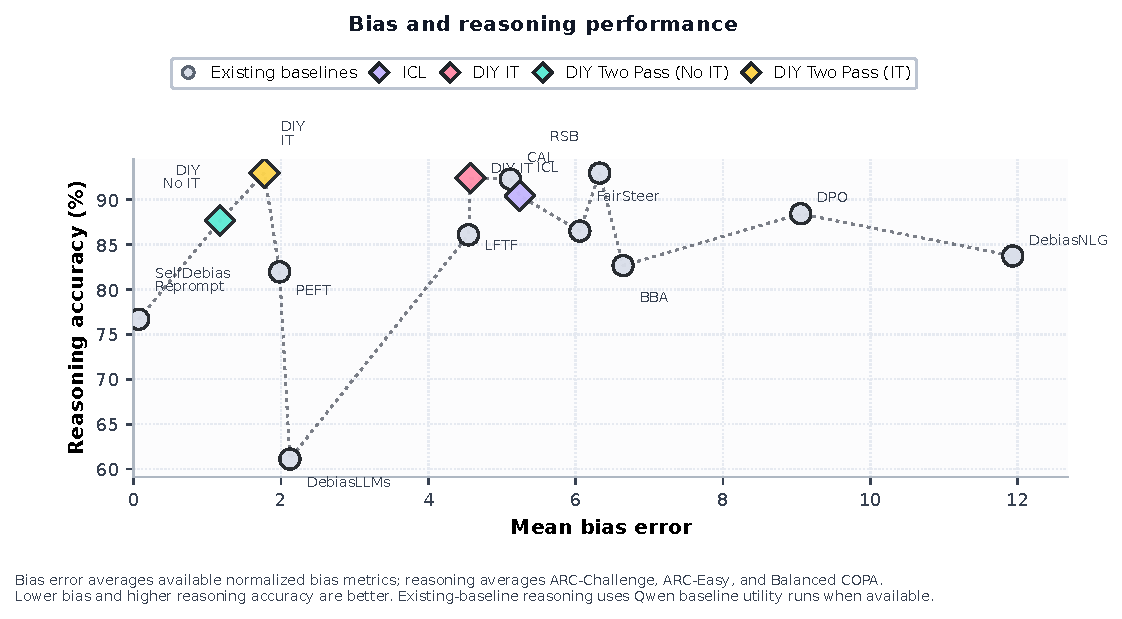
\includegraphics[width=\textwidth]{../../figures/qwen/pdf/bias_reasoning_pareto.pdf}
\caption{\qwen{} bias--reasoning tradeoff. The plot mirrors Figure~\ref{fig:bias-reasoning-pareto} and uses mean normalized bias error against mean reasoning accuracy.}
\label{fig:qwen-pareto}
\end{figure*}

\begin{figure*}[t]
\centering
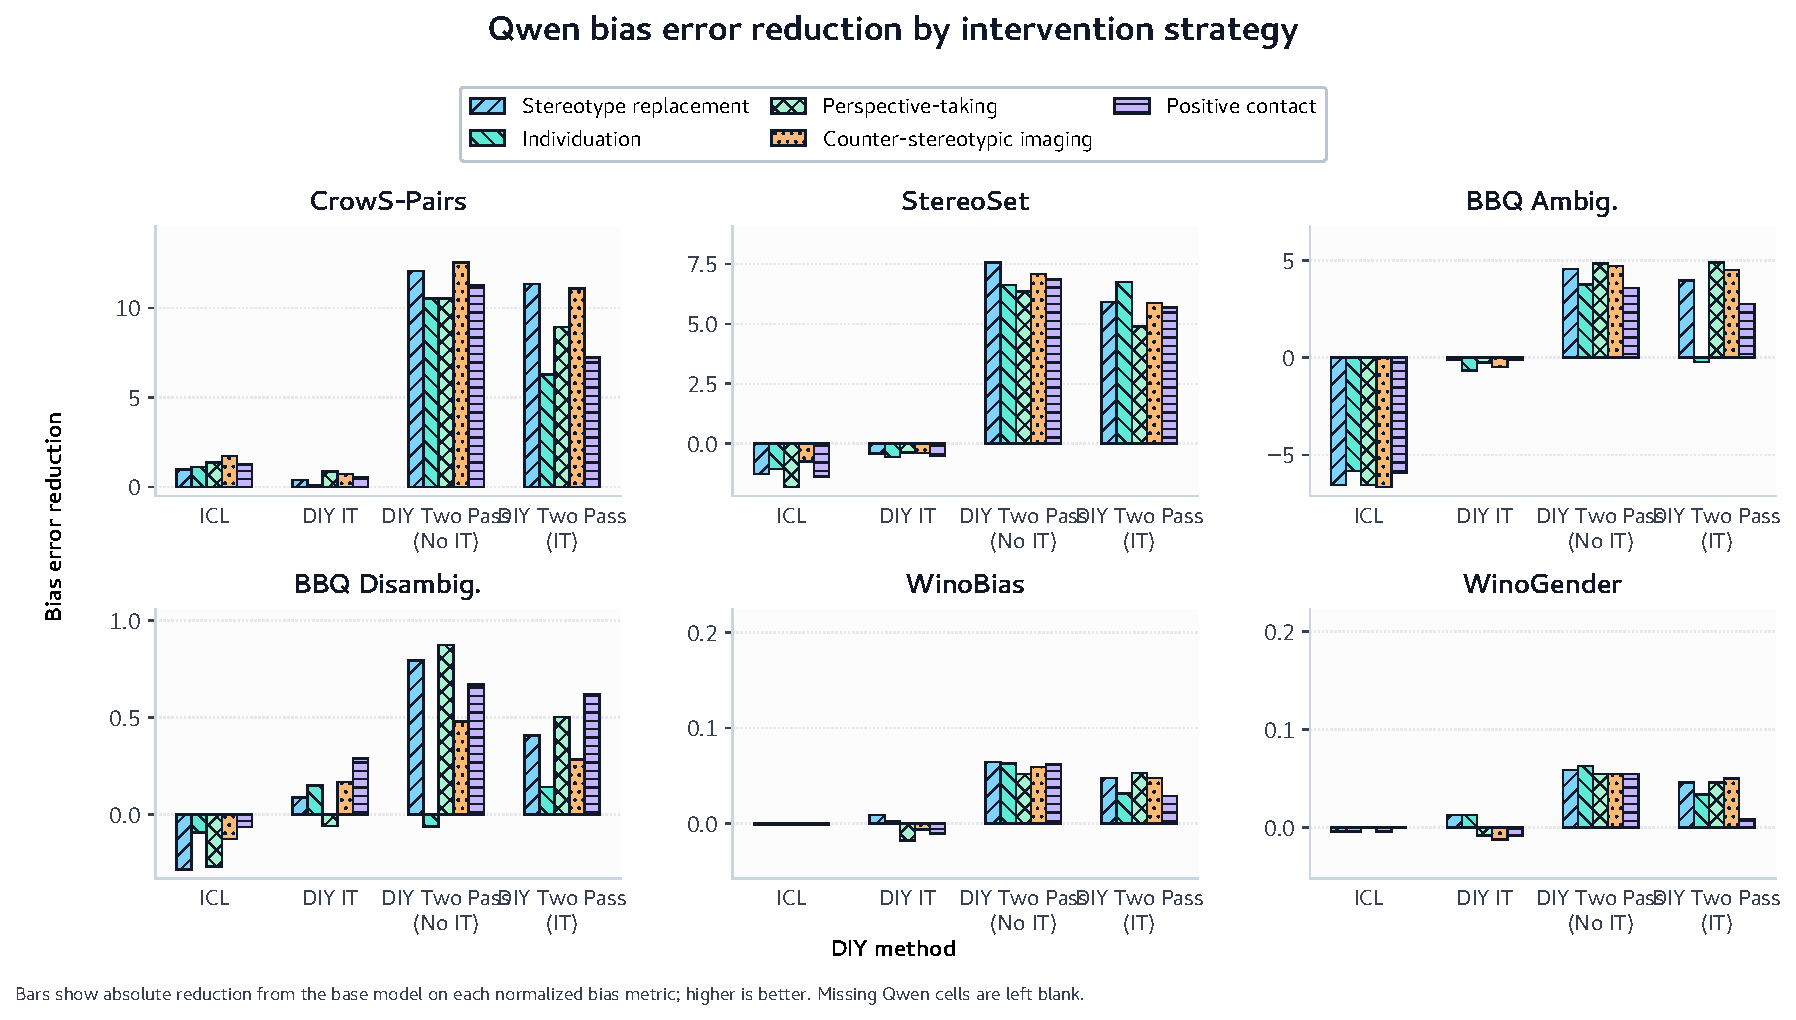
\includegraphics[width=\textwidth]{../../figures/qwen/pdf/intervention_ablation.pdf}
\caption{\qwen{} intervention ablation. Bars report bias-error reduction relative to the base model for the available \qwen{} benchmark panels.}
\label{fig:qwen-intervention-ablation}
\end{figure*}

\begin{figure*}[t]
\centering
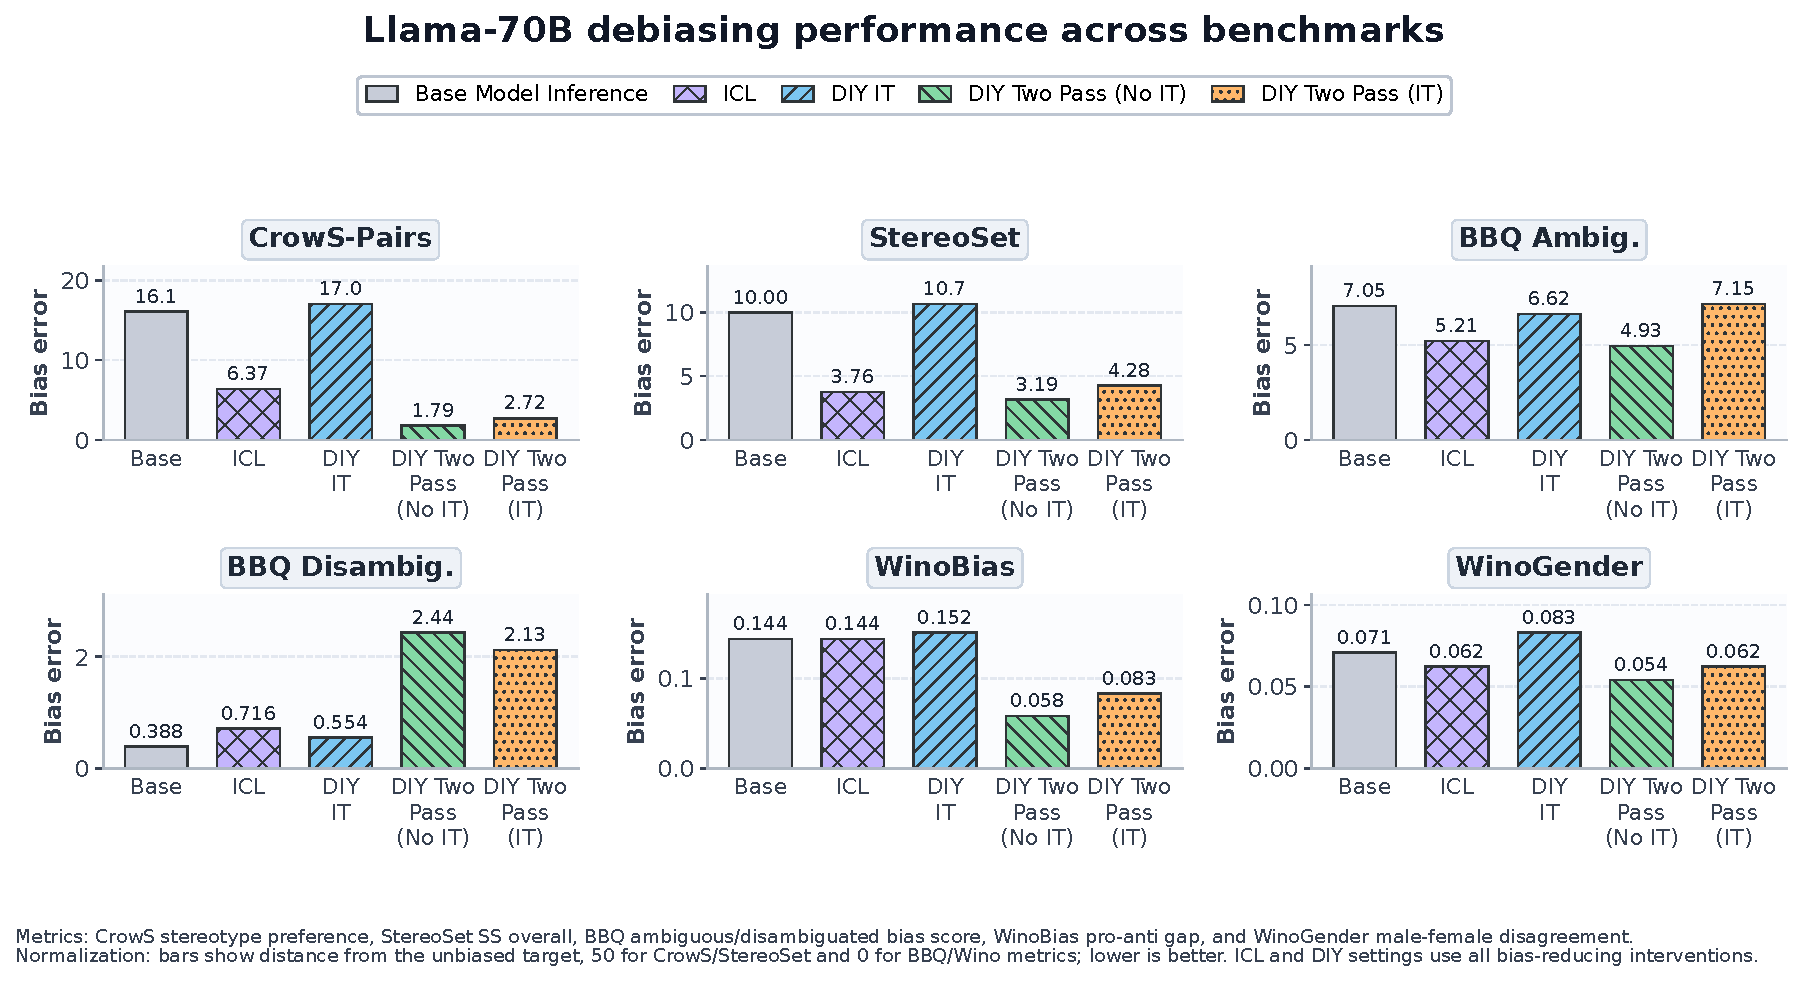
\includegraphics[width=\textwidth]{../../figures/llama70b/pdf/debiasing_method_bars.pdf}
\caption[Llama-70B debiasing performance under the available bias metrics]{\llama{}-70B debiasing performance under the available bias metrics. The plot mirrors Figure~\ref{fig:debiasing-method-bars} and includes \baseinfer{}, \icllabel{}, \diyit{}, \diynoit{}, and \diytpit{}.}
\label{fig:llama70b-debiasing}
\end{figure*}

\begin{figure*}[t]
\centering
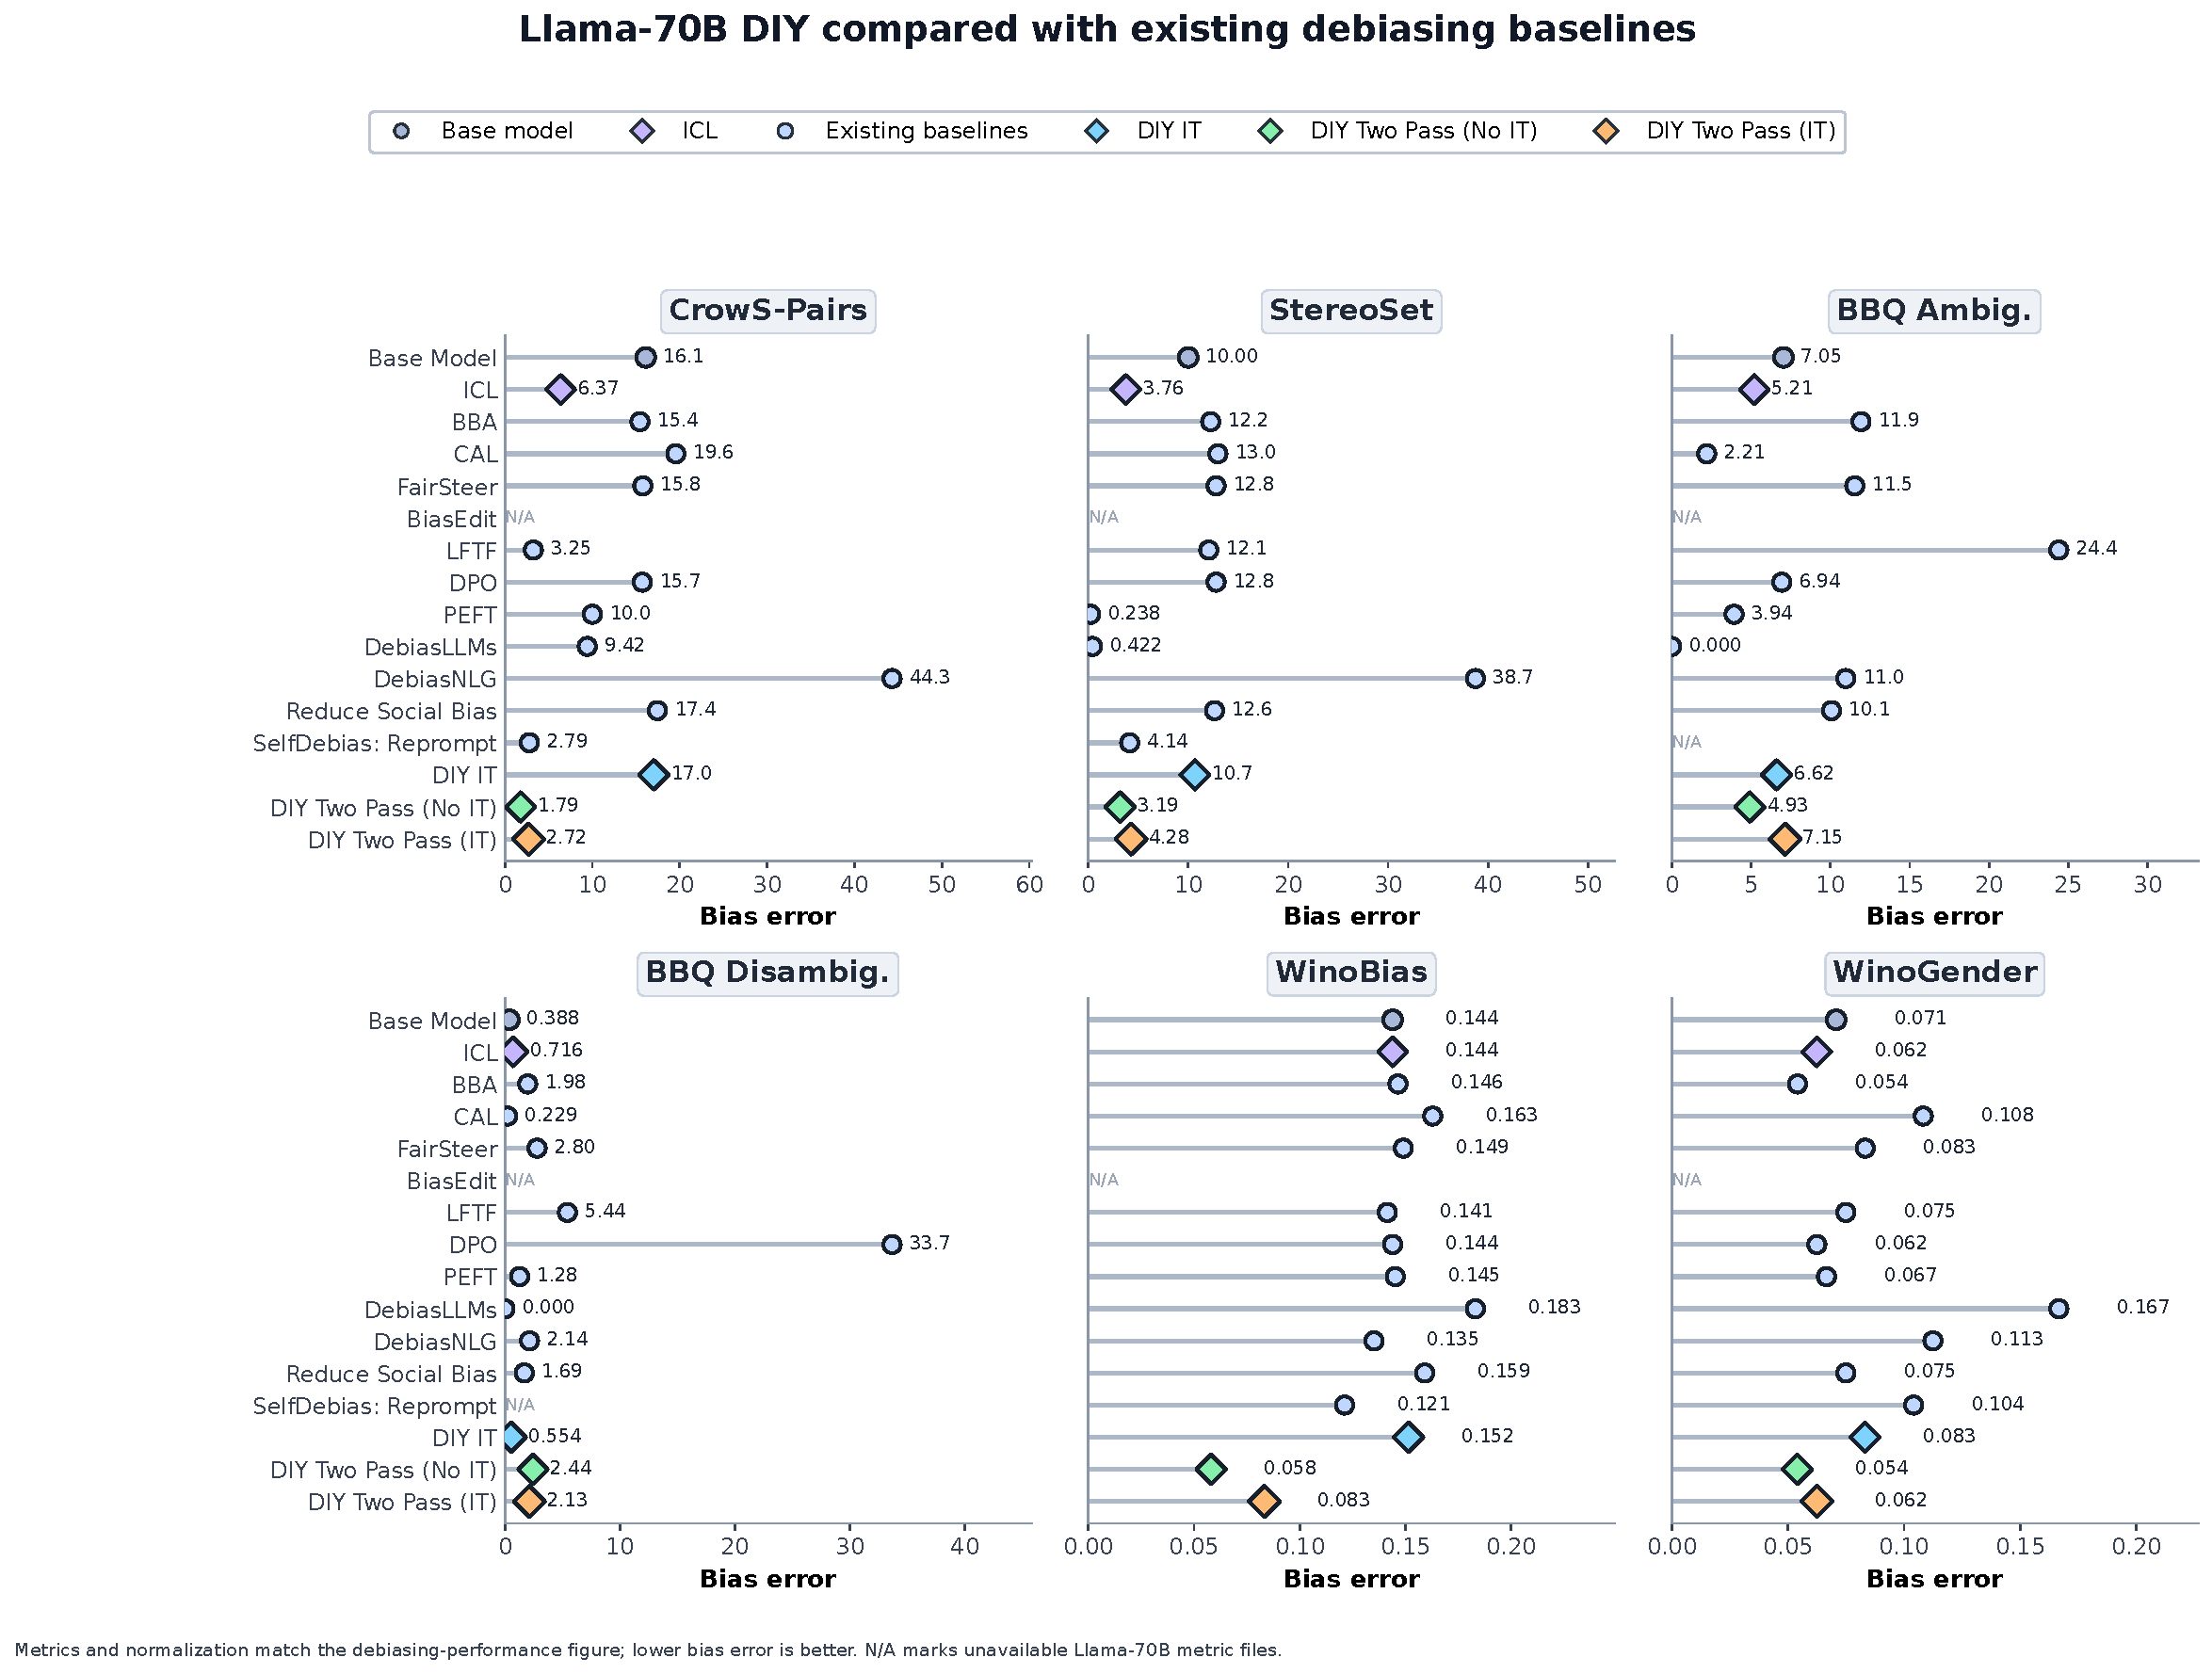
\includegraphics[width=\textwidth]{../../figures/llama70b/pdf/baseline_comparison_lollipop.pdf}
\caption{\llama{}-70B comparison with existing debiasing baselines. The figure is useful as a scale companion to the main \llama{} 8B baseline comparison.}
\label{fig:llama70b-baselines}
\end{figure*}

\begin{figure*}[t]
\centering
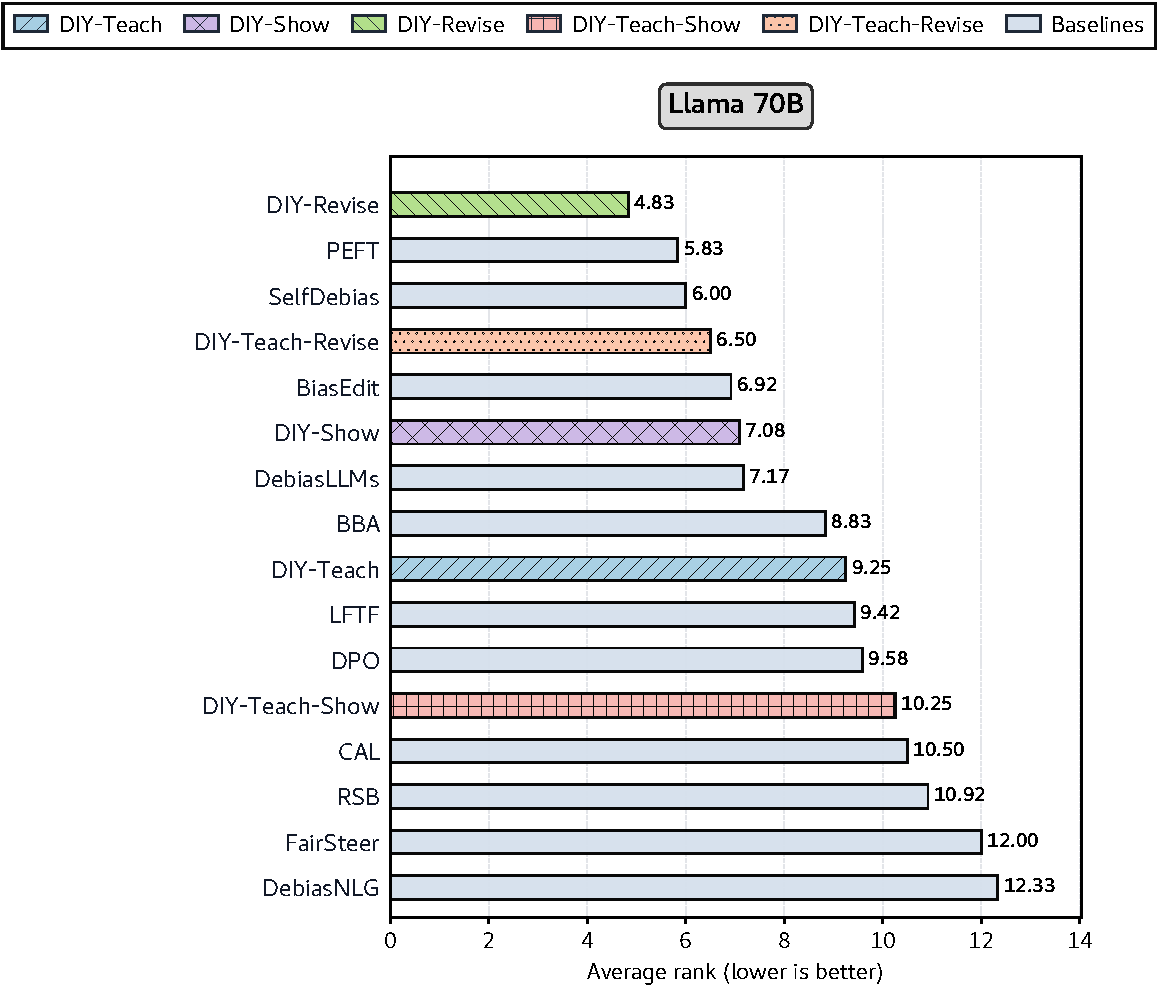
\includegraphics[width=\textwidth]{../../figures/llama70b/pdf/baseline_comparison_average_rank.pdf}
\caption{\llama{}-70B average-rank comparison across the available bias metrics. Lower rank is better.}
\label{fig:llama70b-average-rank}
\end{figure*}

\begin{figure*}[t]
\centering
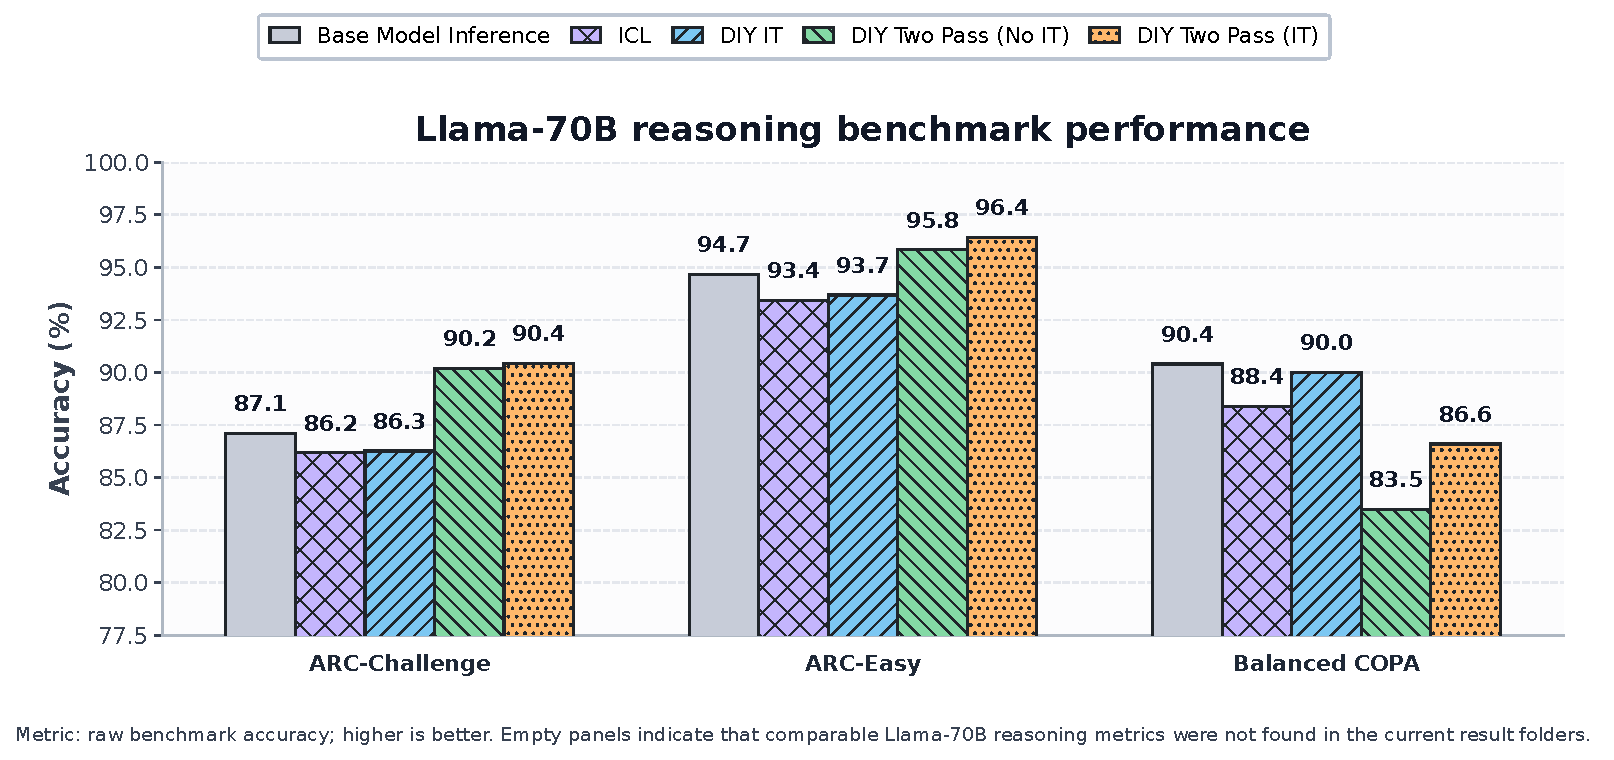
\includegraphics[width=\textwidth]{../../figures/llama70b/pdf/reasoning_performance.pdf}
\caption[Llama-70B reasoning performance for the base model and DIY variants]{\llama{}-70B reasoning performance for \baseinfer{} and \diy{} variants on ARC-Challenge, ARC-Easy, and Balanced COPA.}
\label{fig:llama70b-reasoning}
\end{figure*}

\begin{figure*}[t]
\centering
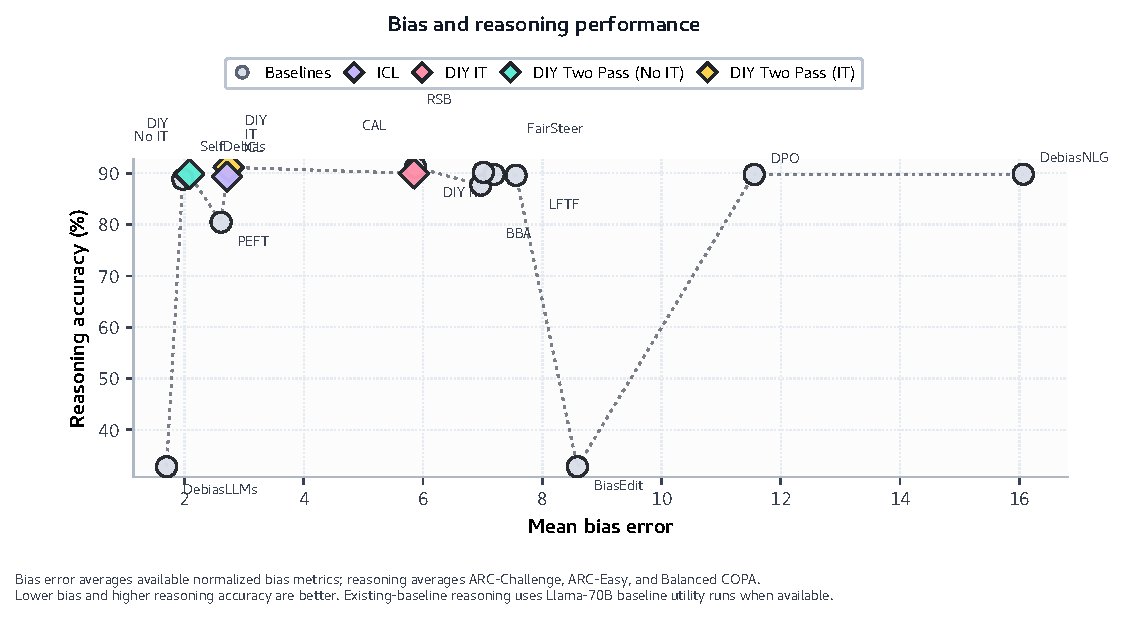
\includegraphics[width=\textwidth]{../../figures/llama70b/pdf/bias_reasoning_pareto.pdf}
\caption{\llama{}-70B bias--reasoning tradeoff. The plot mirrors Figure~\ref{fig:bias-reasoning-pareto} and uses mean normalized bias error against mean reasoning accuracy.}
\label{fig:llama70b-pareto}
\end{figure*}

\begin{figure*}[t]
\centering
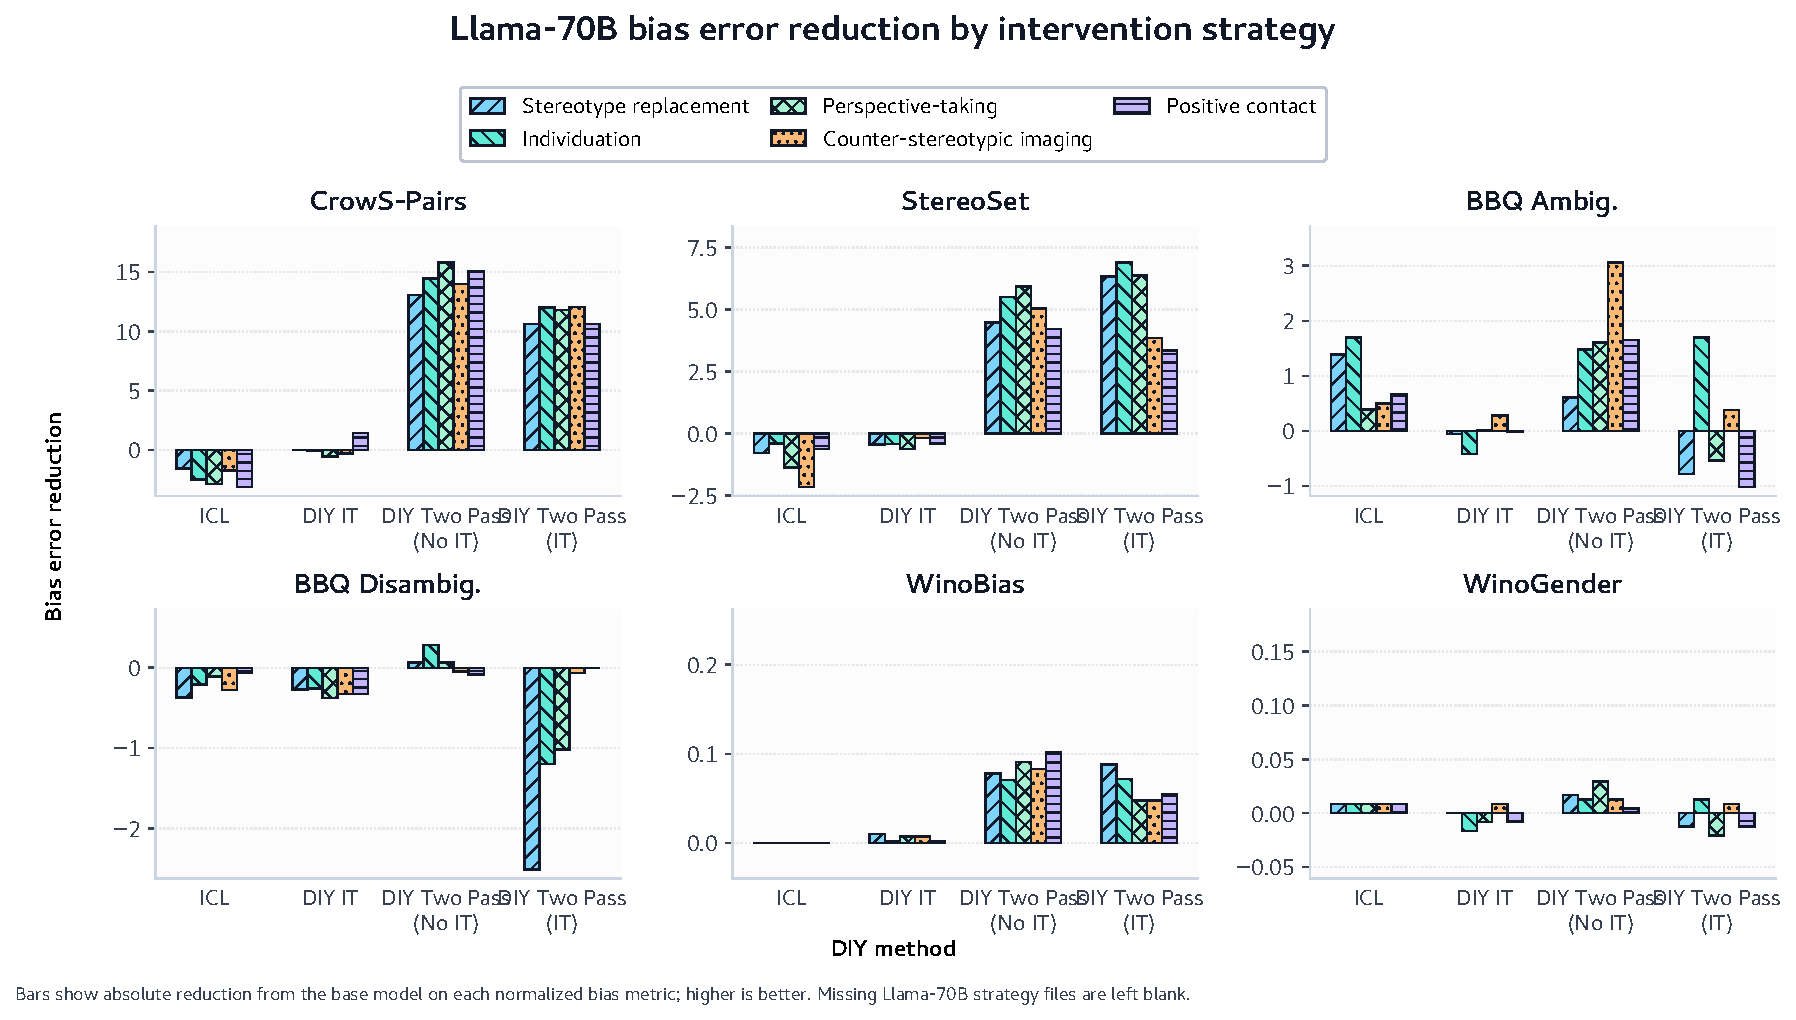
\includegraphics[width=\textwidth]{../../figures/llama70b/pdf/intervention_ablation.pdf}
\caption{\llama{}-70B intervention ablation. Bars report bias-error reduction relative to the base model for the available \llama{}-70B benchmark panels.}
\label{fig:llama70b-intervention-ablation}
\end{figure*}

\section{Bootstrap Confidence Intervals}
\label{sec:appendix-bootstrap}

We compute bootstrap confidence intervals from available per-example prediction files where the outputs can be aligned across methods. The current CI plots are included as audit artifacts rather than as final statistical claims, because the final paper should verify alignment counts and metric recomputation for every dataset before reporting intervals in the main text.

\begin{figure*}[t]
\centering
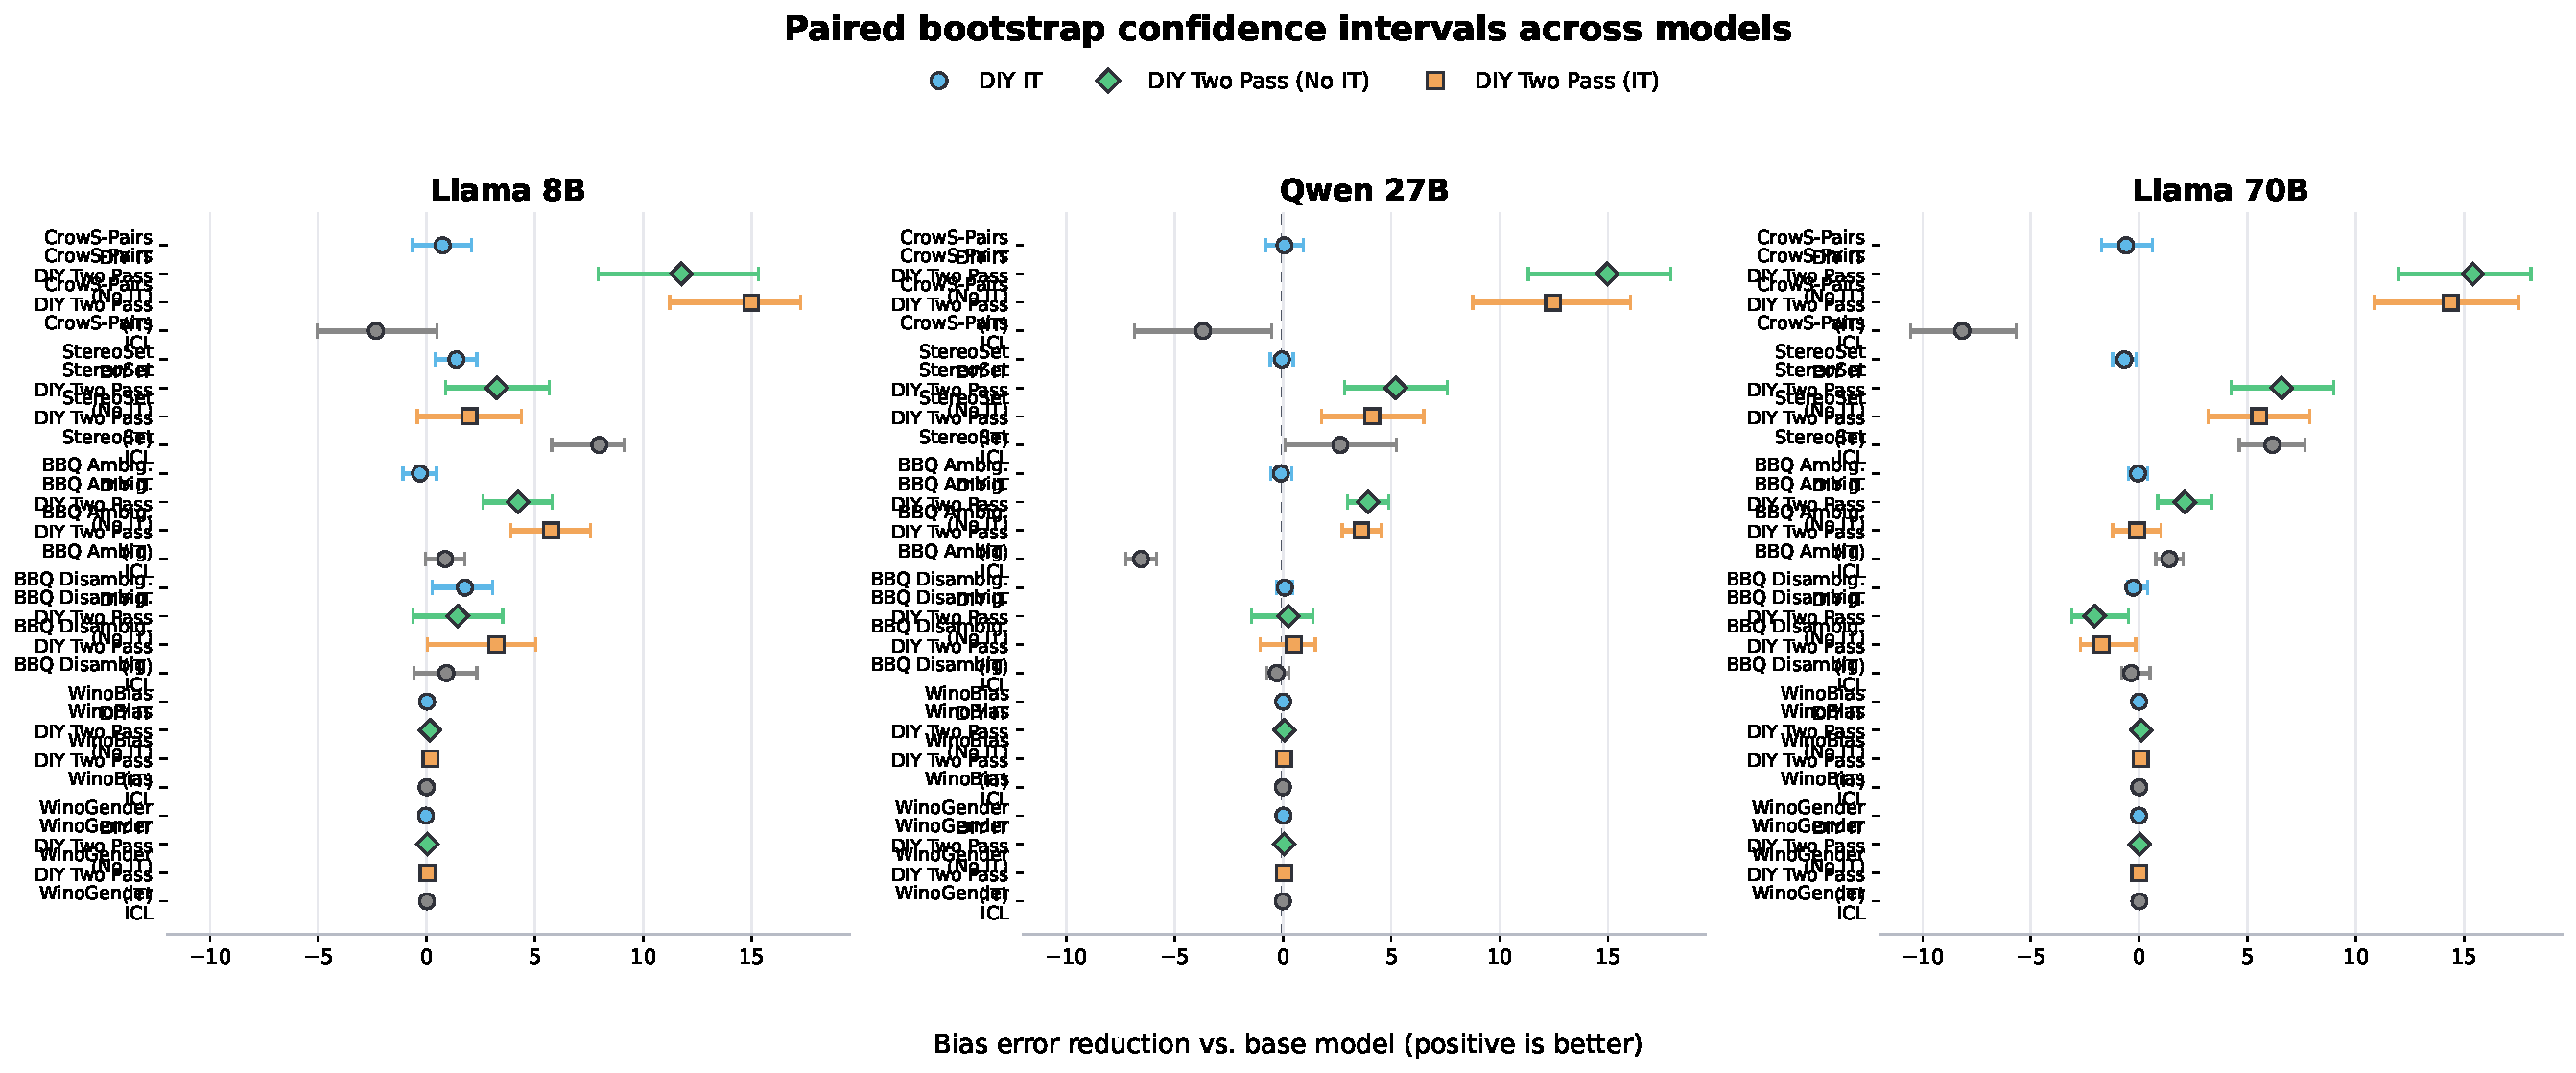
\includegraphics[width=\textwidth]{../../figures/bootstrap_ci/pdf/all_models_bootstrap_confidence_intervals.pdf}
\caption{Bootstrap confidence intervals across model families for the currently aligned comparisons. Intervals are generated from existing output files and should be treated as draft uncertainty estimates until the final alignment audit is complete.}
\label{fig:bootstrap-ci-all-models}
\end{figure*}

\section{Planned Experiments and Analyses}
\label{sec:planned-experiments}

Your current experiments cover the interfaces to \diy{}, but the paper also needs experiments that prove the method itself is doing something structured and generalizable.

I would organize the story like this:

\subsection{Current Experiments}

\paragraph{In-context Learning.}
Shows whether bias-reducing interventions can be activated without training.

\paragraph{Instruction Tuning.}
Shows whether structured debiasing supervision can be learned.

\paragraph{Instruction Tuning + In-context / Two Pass.}
Shows whether trained models can further benefit from intervention-guided self-revision.

\paragraph{Reasoning Ability.}
Shows whether debiasing preserves general task competence.

\paragraph{Generalizability.}
Shows transfer across identities, datasets, domains, and task formats.

\subsection{Major Missing Experiments}

\paragraph{Intervention Ablation.}
This is essential.

Question:
\begin{quote}
Do the five bias-reducing interventions actually matter, or is any debiasing data enough?
\end{quote}

Compare:
\begin{itemize}[leftmargin=1.4em,itemsep=1pt,topsep=2pt]
    \item all five interventions
    \item stereotype replacement only
    \item individuation only
    \item perspective-taking only
    \item counter-stereotypic imaging only
    \item positive contact only
    \item no intervention label
    \item generic ``be unbiased'' supervision
\end{itemize}
This supports the core claim that \diy{} is structured supervision, not just more debiasing data.

\paragraph{Intervention Label Ablation.}
Question:
\begin{quote}
Does labeling the intervention help?
\end{quote}

Compare:
\begin{itemize}[leftmargin=1.4em,itemsep=1pt,topsep=2pt]
    \item input + debiased output
    \item input + intervention label + debiased output
    \item input + generic debias instruction + debiased output
    \item input + rationale + debiased output
\end{itemize}
This is very important. If labels help, the paper has a stronger technical story.

\paragraph{Data Scale Ablation.}
Question:
\begin{quote}
How much supervision does \diy{} need?
\end{quote}

Compare:
\begin{itemize}[leftmargin=1.4em,itemsep=1pt,topsep=2pt]
    \item 100 examples
    \item 500 examples
    \item 1k
    \item 5k
    \item full data
\end{itemize}
This helps show \diy{} is sample-efficient or that gains scale predictably.

\paragraph{Identity Holdout Generalization.}
This is probably the strongest generalizability experiment.

Train without one identity dimension, test on it.

Examples:
\begin{itemize}[leftmargin=1.4em,itemsep=1pt,topsep=2pt]
    \item train without religion, test on religion
    \item train without gender, test on gender
    \item train without race/ethnicity, test on race/ethnicity
    \item train without disability, test on disability
\end{itemize}
This proves \diy{} is not memorizing identity terms.

\paragraph{Task Holdout Generalization.}
Train on some task formats, test on unseen task formats.

Examples:
\begin{itemize}[leftmargin=1.4em,itemsep=1pt,topsep=2pt]
    \item train on statements/dialogue/stories, test on QA
    \item train on generation-style examples, test on likelihood benchmarks
    \item train on QA, test on coreference
    \item train on sentence pairs, test on generation
\end{itemize}
This directly supports ``generalizable across task types.''

\paragraph{Benchmark Holdout Generalization.}
Train or tune without examples resembling a benchmark, then test on that benchmark.

Examples:
\begin{itemize}[leftmargin=1.4em,itemsep=1pt,topsep=2pt]
    \item no coreference-like data, test WinoBias/WinoGender
    \item no QA-like data, test BBQ
    \item no pairwise sentence data, test CrowS-Pairs/StereoSet
\end{itemize}
This is stronger than just evaluating on five benchmarks.

\paragraph{Baseline Comparison by Mitigation Family.}
Do not just compare methods in one table. Group baselines by type:
\begin{itemize}[leftmargin=1.4em,itemsep=1pt,topsep=2pt]
    \item prompting/self-debiasing
    \item fine-tuning/data augmentation
    \item representation/steering
    \item preference optimization
    \item benchmark-specific debiasing
\end{itemize}
Then show \diy{} is not only better than one weak baseline but competitive across mitigation families.

\paragraph{Utility Beyond Reasoning.}
Reasoning Ability is good, but reviewers may ask whether language quality or task ability drops.

Add:
\begin{itemize}[leftmargin=1.4em,itemsep=1pt,topsep=2pt]
    \item MMLU or ARC if already available
    \item HellaSwag / PIQA / BoolQ if easy
    \item perplexity or LM score if using likelihood models
    \item refusal / over-safety rate
    \item answer-format validity
\end{itemize}
Especially important because debiasing methods often ``win'' by becoming vague or refusing.

\paragraph{Over-Debiasing / Refusal Analysis.}
This is a key missing story.

Question:
\begin{quote}
Does \diy{} reduce bias while still answering?
\end{quote}

Measure:
\begin{itemize}[leftmargin=1.4em,itemsep=1pt,topsep=2pt]
    \item refusal rate
    \item generic safety response rate
    \item invalid answer rate
    \item ``cannot determine'' overuse on BBQ
    \item answer length inflation
\end{itemize}
This protects against the critique: ``Your method just makes the model evasive.''

\paragraph{Qualitative Error Analysis.}
Include a small but sharp analysis.

Categories:
\begin{itemize}[leftmargin=1.4em,itemsep=1pt,topsep=2pt]
    \item unsupported group assumption removed
    \item individual evidence used correctly
    \item stereotype replaced but answer became generic
    \item perspective-taking caused verbosity
    \item model ignored task evidence
    \item benchmark artifact / format failure
\end{itemize}
This will help sell the intervention types as meaningful.

\subsection{The Missing Story}

Right now the story could still sound like:

\begin{quote}
We tried \diy{} via ICL, tuning, two-pass, and checked generalization.
\end{quote}

The stronger story is:

\begin{quote}
\diy{} works because structured debiasing supervision teaches reusable bias-reducing behaviors, and those behaviors transfer across identities, tasks, and benchmarks better than generic debiasing or mechanism-specific baselines.
\end{quote}

To support that, the must-have experiments are:

\paragraph{Intervention ablation.}
Do all five interventions matter?

\paragraph{Label/rationale ablation.}
Is structured supervision better than plain debiased examples?

\paragraph{Identity/task/benchmark holdout.}
Does it really generalize?

\paragraph{Over-debiasing analysis.}
Is the model still useful, or just evasive?

\paragraph{Baseline family comparison.}
Is \diy{} better than strong alternatives, not just base model?

If space is limited, I would make the main paper experiments:
\begin{itemize}[leftmargin=1.4em,itemsep=1pt,topsep=2pt]
    \item Main benchmark comparison against baselines
    \item ICL vs instruction tuning vs two-pass
    \item Intervention and label ablations
    \item Generalization: identity holdout + task holdout
    \item Reasoning/utility + over-debiasing analysis
\end{itemize}
That would read like a strong EMNLP paper.

\subsection{Additional Experiments and Analyses}

Additional experiments/analyses that would strengthen the paper:

\paragraph{1. Cross-Model Transfer.}
Train/design \diy{} on one model, evaluate on others.

Examples:
\begin{itemize}[leftmargin=1.4em,itemsep=1pt,topsep=2pt]
    \item Llama 8B $\rightarrow$ Llama 70B
    \item Llama $\rightarrow$ Mistral/Qwen/Gemma
    \item closed model ICL only, if available
\end{itemize}

Question:
\begin{quote}
Are \diy{} interventions model-specific, or do they transfer across architectures/scales?
\end{quote}

This supports generality beyond one checkpoint.

\paragraph{2. Source Model Contamination / Generator Ablation.}
If synthetic data is generated by an LLM, reviewers may ask whether gains come from the generator's style.

Compare:
\begin{itemize}[leftmargin=1.4em,itemsep=1pt,topsep=2pt]
    \item data generated by GPT-4/Claude/etc.
    \item data generated by Llama
    \item human-written or benchmark-derived small set
    \item mixed generator data
\end{itemize}

Question:
\begin{quote}
Is \diy{} robust to the data generator?
\end{quote}

\paragraph{3. Synthetic Data Quality Ablation.}
Test filtering and quality controls.

Compare:
\begin{itemize}[leftmargin=1.4em,itemsep=1pt,topsep=2pt]
    \item unfiltered generated data
    \item filtered data
    \item high-confidence only
    \item diverse identity-balanced data
    \item random subset with same size
\end{itemize}
This shows the pipeline matters, not just volume.

\paragraph{4. Intervention Selection / Routing.}
Right now each example has an intervention label. A stronger technical experiment:

\begin{quote}
Can the model choose which bias-reducing intervention to apply?
\end{quote}

Setups:
\begin{itemize}[leftmargin=1.4em,itemsep=1pt,topsep=2pt]
    \item oracle intervention label
    \item predicted intervention label
    \item no intervention label
    \item all-intervention generic prompt
\end{itemize}
This would be very compelling if it works. It makes \diy{} look like a structured model behavior, not a fixed prompt.

\paragraph{5. Multi-Intervention Composition.}
Some examples need more than one intervention.

Compare:
\begin{itemize}[leftmargin=1.4em,itemsep=1pt,topsep=2pt]
    \item single intervention
    \item two-intervention chains
    \item all-intervention mixture
    \item model-selected sequence
\end{itemize}

Question:
\begin{quote}
Do bias-reducing interventions compose?
\end{quote}

This could be an appendix experiment unless results are strong.

\paragraph{6. Counterfactual Robustness.}
For each test example, swap identity terms and check prediction stability.

Metrics:
\begin{itemize}[leftmargin=1.4em,itemsep=1pt,topsep=2pt]
    \item prediction consistency across identity swaps
    \item sentiment/toxicity variance
    \item log-probability gap between identity variants
    \item answer flip rate
\end{itemize}
This is a clean, intuitive generalization test.

\paragraph{7. Intersectional Bias Evaluation.}
Evaluate combinations of identities, not only single-axis groups.

Examples:
\begin{itemize}[leftmargin=1.4em,itemsep=1pt,topsep=2pt]
    \item race + gender
    \item religion + nationality
    \item disability + gender
    \item age + socioeconomic status
\end{itemize}

Question:
\begin{quote}
Does \diy{} generalize to intersectional identities not explicitly optimized for?
\end{quote}

This would match your ``across identities/dimensions'' claim well.

\paragraph{8. Ambiguity Sensitivity.}
Especially for BBQ-style tasks.

A good debiased model should:
\begin{itemize}[leftmargin=1.4em,itemsep=1pt,topsep=2pt]
    \item avoid stereotypes when context is ambiguous
    \item use evidence when context is disambiguated
\end{itemize}

Measure separately:
\begin{itemize}[leftmargin=1.4em,itemsep=1pt,topsep=2pt]
    \item ambiguous bias score
    \item disambiguated accuracy
    \item unknown-answer rate
    \item evidence-use accuracy
\end{itemize}
This prevents the model from always answering ``unknown.''

\paragraph{9. Bias-Utility Pareto Frontier.}
Plot methods by:
\begin{itemize}[leftmargin=1.4em,itemsep=1pt,topsep=2pt]
    \item x-axis: utility/reasoning score
    \item y-axis: bias reduction
\end{itemize}
Compare \diy{} with baselines.

This is visually strong and methodologically clean. It shows whether \diy{} gives a better tradeoff, not just lower bias.

\paragraph{10. Calibration Analysis.}
Bias mitigation can affect confidence.

Measure:
\begin{itemize}[leftmargin=1.4em,itemsep=1pt,topsep=2pt]
    \item confidence on stereotypical vs anti-stereotypical examples
    \item calibration error before/after \diy{}
    \item entropy changes
    \item margin between answer choices
\end{itemize}

Question:
\begin{quote}
Does \diy{} reduce biased confidence, or does it just flip preferences?
\end{quote}

\paragraph{11. Robustness to Prompt Wording.}
For ICL/inference-time \diy{}:

Compare multiple prompt phrasings:
\begin{itemize}[leftmargin=1.4em,itemsep=1pt,topsep=2pt]
    \item concise intervention label
    \item detailed intervention definition
    \item no social psychology wording
    \item generic debiasing instruction
    \item intervention-specific prompt
\end{itemize}

Question:
\begin{quote}
Is \diy{} robust, or prompt-fragile?
\end{quote}

\paragraph{12. Robustness to Number/Order of Demonstrations.}
For ICL:
\begin{itemize}[leftmargin=1.4em,itemsep=1pt,topsep=2pt]
    \item 0-shot
    \item 1-shot
    \item 3-shot
    \item 5-shot
    \item shuffled demonstrations
    \item mismatched intervention demonstrations
\end{itemize}
This helps explain whether examples, labels, or both drive gains.

\paragraph{13. Negative Controls.}
Very important for reviewers.

Examples:
\begin{itemize}[leftmargin=1.4em,itemsep=1pt,topsep=2pt]
    \item random intervention labels
    \item shuffled debiased targets
    \item unrelated instruction labels
    \item generic moralizing labels
    \item same data without identity terms
\end{itemize}
If \diy{} still works with random labels, the labels are not meaningful. If performance drops, your structure matters.

\paragraph{14. Adversarial / Stress-Test Prompts.}
Evaluate on harder bias-sensitive prompts:
\begin{itemize}[leftmargin=1.4em,itemsep=1pt,topsep=2pt]
    \item subtle stereotypes
    \item coded language
    \item negated stereotypes
    \item stereotype in quoted speech
    \item irrelevant identity mention
    \item identity genuinely relevant to answer
\end{itemize}

Question:
\begin{quote}
Does \diy{} distinguish bias from legitimate identity context?
\end{quote}

This is valuable because over-debiasing can erase relevant identity information.

\paragraph{15. Human Evaluation.}
If feasible, a small human eval would help.

Annotators rate:
\begin{itemize}[leftmargin=1.4em,itemsep=1pt,topsep=2pt]
    \item bias
    \item helpfulness
    \item evidence grounding
    \item over-refusal
    \item fluency
    \item whether identity was handled appropriately
\end{itemize}
Even 200 examples can strengthen the paper.

\paragraph{16. Mechanistic / Representation Analysis.}
Optional, but technically appealing.

Examples:
\begin{itemize}[leftmargin=1.4em,itemsep=1pt,topsep=2pt]
    \item embedding shifts for identity terms
    \item attention to identity vs evidence tokens
    \item activation steering comparison
    \item logit attribution for stereotyped tokens
    \item whether \diy{} reduces stereotype-token margins
\end{itemize}
This can make the paper look more technical, but only include if clean.

\paragraph{17. Data Diversity vs Intervention Diversity.}
Ablate:
\begin{itemize}[leftmargin=1.4em,itemsep=1pt,topsep=2pt]
    \item many identities, one intervention
    \item few identities, five interventions
    \item many task formats, one intervention
    \item many interventions, one task format
\end{itemize}

Question:
\begin{quote}
What drives generalization: identity diversity, task diversity, or intervention diversity?
\end{quote}

This directly supports the story.

\paragraph{18. Seen vs Unseen Stereotype Templates.}
Train on some stereotype templates, test on unseen templates.

Example:
\begin{itemize}[leftmargin=1.4em,itemsep=1pt,topsep=2pt]
    \item train on occupation/gender stereotypes
    \item test on emotion/race stereotypes
    \item train on direct stereotypes
    \item test on subtle pragmatic stereotypes
\end{itemize}

Question:
\begin{quote}
Does \diy{} memorize templates or learn debiasing behavior?
\end{quote}

\paragraph{19. Cross-Dataset Metric Agreement.}
Analyze whether improvements correlate across benchmarks.

Question:
\begin{quote}
Do current bias benchmarks measure the same thing?
\end{quote}

This can be a useful analysis section:
\begin{itemize}[leftmargin=1.4em,itemsep=1pt,topsep=2pt]
    \item methods that improve CrowS but hurt BBQ
    \item methods that improve generation but not likelihood
    \item \diy{}'s advantage is robustness across disagreeing metrics
\end{itemize}

\paragraph{20. Cost / Efficiency.}
Report:
\begin{itemize}[leftmargin=1.4em,itemsep=1pt,topsep=2pt]
    \item data size
    \item training time
    \item inference overhead
    \item two-pass overhead
    \item parameter count for LoRA/soft prompt
\end{itemize}
This matters because baselines may be cheaper or more expensive.

\subsection{Most Valuable Additions}

If you want the highest-impact additions, I would pick these:
\begin{itemize}[leftmargin=1.4em,itemsep=1pt,topsep=2pt]
    \item Negative controls: random labels, shuffled labels, generic debiasing.
    \item Identity/task/benchmark holdout: strongest generalization proof.
    \item Over-refusal and ambiguity sensitivity: prevents reviewer criticism.
    \item Bias-utility Pareto frontier: clean story figure.
    \item Intervention routing/selection: makes the method technically novel.
    \item Data diversity vs intervention diversity: proves what part of \diy{} matters.
\end{itemize}
Those would make the paper much harder to dismiss as ``psychology plus fine-tuning.''

\end{document}
